\documentclass{beamer}
%\documentclass[serif]{beamer}


\mode<presentation>
{
% \usetheme{Warsaw}
%  \usetheme{Madrid}
 \usetheme{Boadilla}

  \setbeamercovered{transparent}
}


\usepackage[english]{babel}
\usepackage[utf8]{inputenc}
\usepackage{times}
\usepackage[T1]{fontenc}

\usepackage{xcolor}
\usepackage{colortbl}
\usepackage{subfigure}
\usepackage{CJK}

% Or whatever. Note that the encoding and the font should match. If T1
% does not look nice, try deleting the line with the fontenc.
%%%%%%%%%%%%%%%%%%%%%%%%%%%%%%%%%%%%%%%%%%%%%%%%%%%%%%%%%%%%%%%%%%%%%%
%% abbreviations

%% for tables
\newcommand{\mc}{\multicolumn}
\newcommand{\lab}[1]{\multicolumn{1}{c}{#1}}
\newcommand{\ind}[1]{{\fboxsep1pt\raisebox{-.5ex}{\fbox{{\tiny #1}}}}}

%% for dcolumn
%\newcolumntype{d}{D{.}{.}{1.4}}
%\newcolumntype{s}{D{.}{.}{0.3}}

%% markup
%\renewcommand{\key}[1]{\alert{\textit{#1}}}
\newcommand{\buffer}[1]{{\color{blue}\textbf{#1}}}
\newcommand{\pred}[1]{\code{#1}}

%% colors
\newcommand{\textred}[1]{\alert{#1}}
\newcommand{\textblue}[1]{\buffer{#1}}
\definecolor{tablecolor}{cmyk}{0,0.3,0.3,0}
\newcommand{\keytab}[1]{\mc{1}{>{\columncolor{tablecolor}}d}{#1}}

% rules
\newcommand{\psr}[2]{#1 $\rightarrow \langle $ #2 $\rangle$}

\newenvironment{unpacked_itemize}{
\begin{itemize}
  \setlength{\itemsep}{10pt}
  \setlength{\parskip}{0pt}
  \setlength{\parsep}{0pt}
}{\end{itemize}}

\newcommand{\condon}{\hspace{0pt} | \hspace{1pt}}
\definecolor{darkblue}{rgb}{0,0,0.6}
\newcommand{\blueexample}[1]{\textcolor{darkblue}{\rm #1}}

%%%%%%%%%%%%%%%%%%%%%%%%%%%%%%%%%%%%%%%%%%%%%%%%%%%%%%%%%%%%%%%%%%%%%%

\newcommand{\bx}{\mathbf{x}}
\newcommand{\bz}{\mathbf{z}}
\newcommand{\bd}{\mathbf{d}}
\newcommand{\by}{\mathbf{y}}
\newcommand\bleu{${B{\scriptstyle LEU}}$}


\title[A Note on the Implemention of HDPs]{A Note on the Implementation of Hierarchical Dirichlet Processes}

\author[Blunsom et al.]{{\bf Phil Blunsom}$^*$, Trevor Cohn$^*$, \\Sharon
Goldwater$^*$ and Mark Johnson$^\dagger$}

\institute[Uni. of Edinburgh] % (optional, but mostly needed)
{
  $^*$School of Informatics, University of Edinburgh \\
  $^\dagger$Department of Cognitive and Linguistic Sciences, Brown University \\
}

\date{August 4, 2009}


\subject{Hierarchical Dirichlet Processes}


\pgfdeclareimage[height=1.0cm]{university-logo}{logo}
\logo{\pgfuseimage{university-logo}}

\AtBeginSection[]
{
  \begin{frame}<beamer>{Outline}
    %\tableofcontents[currentsection,currentsubsection]
    \tableofcontents[currentsection]
  \end{frame}
}


%\beamerdefaultoverlayspecification{<+->}


\begin{document}

\begin{frame}
  \titlepage
\end{frame}


\begin{frame}[t]{Outline}
%\begin{exampleblock}{An example}
\vspace{0.5in}
\Large
\begin{unpacked_itemize}
\onslide<1-> \item GGJ06\footnote{S. Goldwater, T. Griffiths, M. Johnson.
Contextual dependencies in unsupervised word segmentation. ACL/COLING-06} 
introduced an approximation for use in hierarchical Dirichlet process (HDP) inference: \\ 
\onslide<2->{\alert{\textbf{It's wrong, don't use it.}}}
\onslide<3-> \item We correct that approximation for DP models. \\ 
\onslide<4->{\alert{\textbf{However, this doesn't extend to HDPs.}}}
\onslide<5> \item But that's ok because we'll describe an efficient exact implementation.
\end{unpacked_itemize}
%\end{exampleblock}
\end{frame}

\begin{frame}
\frametitle{The Chinese Restaurant Process}
In a Dirichlet Process unigram language model  words $w_1 \ldots w_n$ are generated as follows: 
\begin{align}
\nonumber G | & \alpha_0, P_0 &\sim & ~ \mbox{DP}(\alpha_0,P_0) \\
\nonumber w_i | & G &\sim & ~ G 
\end{align}
\begin{itemize}
  \item $G$ is a distribution over an infinite set of words, 
  \item $P_0$ is the probability that an word will be in the support of $G$, 
  \item $\alpha_0$ determines the variance of $G$.
\end{itemize}
\vspace{0.2in}
One way of understanding the predictions made by the DP model is through the Chinese restaurant process (CRP) \dots
\end{frame}

\begin{frame}
\frametitle{The Chinese Restaurant Process}
\only<1-9>{\vspace{-0.4in}}
\begin{figure}
\begin{center}
  \only<1>{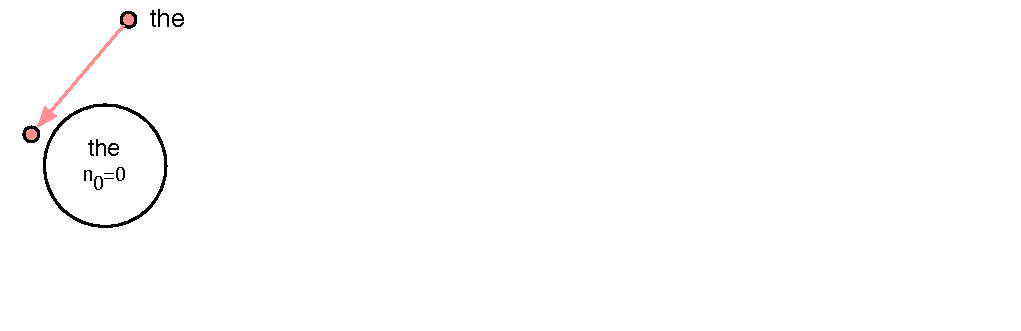
\includegraphics[scale=0.7]{tables0.pdf}}
  \only<2>{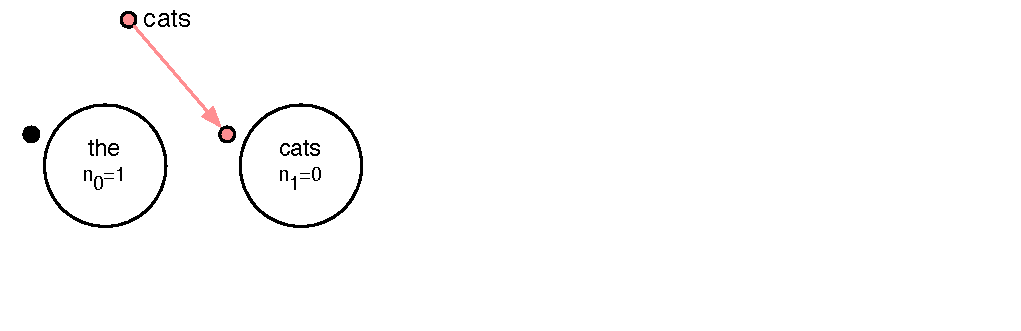
\includegraphics[scale=0.7]{tables1.pdf}}
  \only<3>{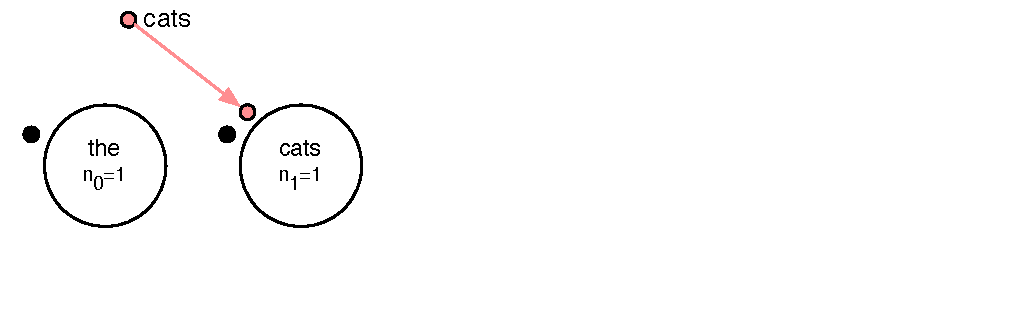
\includegraphics[scale=0.7]{tables2.pdf}}
  \only<4>{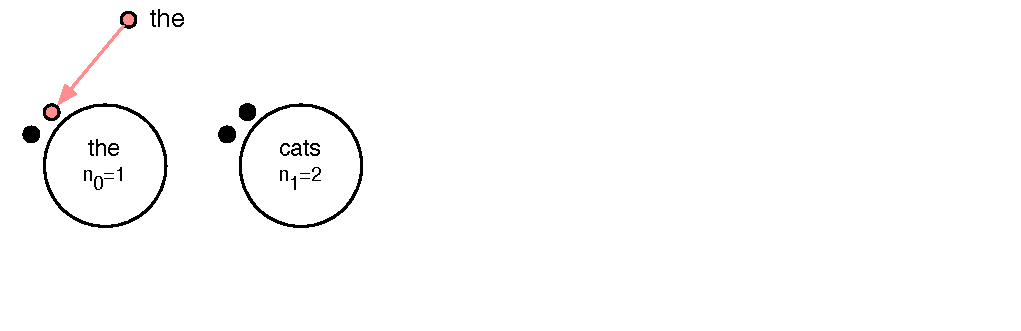
\includegraphics[scale=0.7]{tables3.pdf}}
  \only<5>{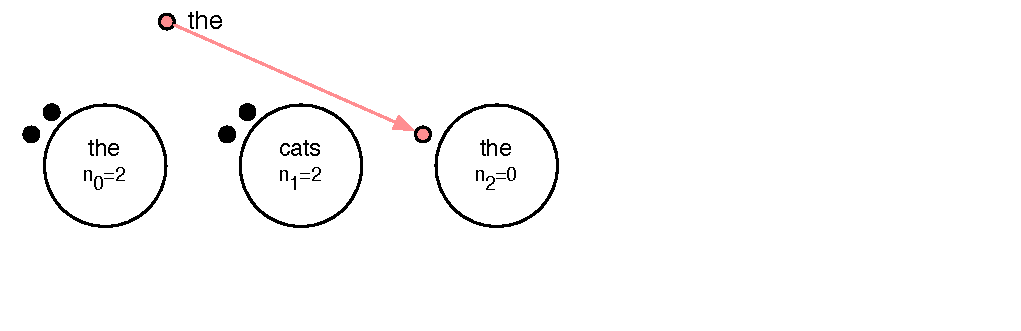
\includegraphics[scale=0.7]{tables4.pdf}}
  \only<6>{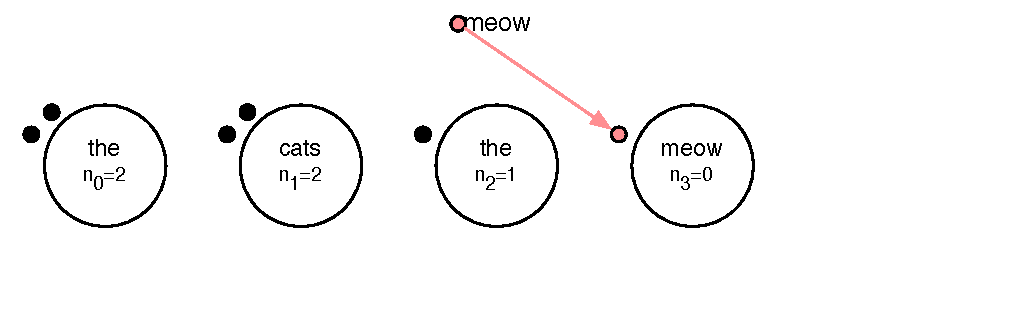
\includegraphics[scale=0.7]{tables5.pdf}}
  \only<7>{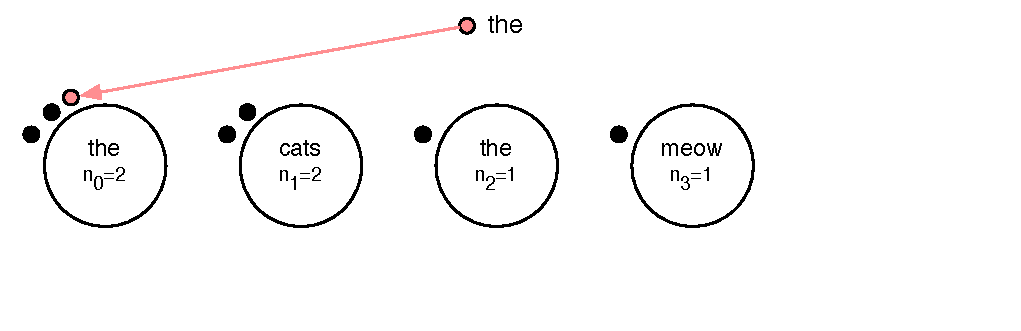
\includegraphics[scale=0.7]{tables7.pdf}}
  \only<8>{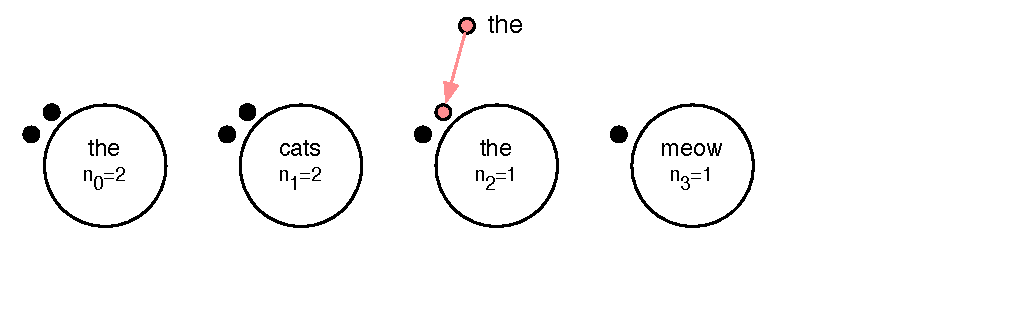
\includegraphics[scale=0.7]{tables8.pdf}}
  \only<9>{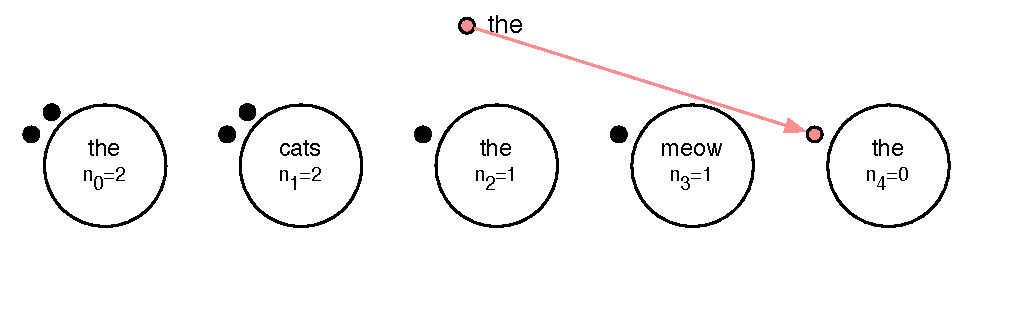
\includegraphics[scale=0.7]{tables6.pdf}}
\end{center}
\end{figure}
\only<1-6>{
\vspace{-0.6in}
Customers (words) enter a restaurant and choose a table according to the distribution:
\begin{align}
\nonumber P(z_i = k | w_i = w, \mathbf{z}_{-i}) = \left\{ 
\begin{array}{ll} 
  \frac{n_k^{\mathbf{z}_{-i}}}{n_w + \alpha_0 P_0(w)}, 0 \leq k < |k|  \\
  \\ \frac{\alpha_0 P_0(w)}{n_w + \alpha_0 P_0(w)}, k = |k|
\end{array} \right.
\end{align}
%where $\mathbf{z}_{-i} = z_1 \dots z_{i-1}$ are the table assignments of the previous customers, $n_k^{\mathbf{z}_{-i}}$ is the number of customers at table $k$ in ${\mathbf{z}_{-i}}$, and $K(\mathbf{z}_{-i})$ is the total number of occupied tables.  
}
\only<7-9>{
\vspace{-0.4in}
The 7$^{th}$ customer `{\em the}' enters the restaurant and choses a table from
those already seating `{\em the}', or opening a new table:
}
\only<7>{
\begin{align}
\nonumber P(z_6 = 0 | w_6 = the, \mathbf{z}_{-6}) = \frac{2}{3 + \alpha_0 P_0(the)}
\end{align}
}
\only<8>{
\begin{align}
\nonumber P(z_6 = 2 | w_6 = the, \mathbf{z}_{-6}) = \frac{1}{3 + \alpha_0 P_0(the)}
\end{align}
}
\only<9>{
\begin{align}
\nonumber P(z_6 = 4 | w_6 = the, \mathbf{z}_{-6}) = \frac{P_0(the)}{3 + \alpha_0 P_0(the)}
\end{align}
}
\only<7-9>{\vspace{0.32in}}
\end{frame}

\begin{frame}
\frametitle{Approximating the table counts}
\begin{figure}
\begin{center}
  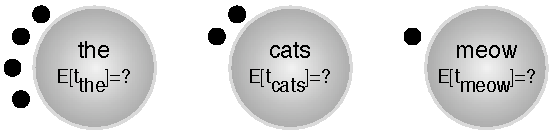
\includegraphics[scale=0.7]{tables_expectation.pdf}
\end{center}
\end{figure}

\begin{itemize}
  \item GGJ06 sought to avoid explicitly tracking tables by reasoning under
the expected table counts ($E[t_w]$).

\item Antoniak(1974) derives the expected table count as equal to the recurrence:
\begin{align}
\nonumber E[t_w] = \alpha_0 P_0(w) \sum_{i=1}^{n_w} \frac{1}{\alpha_0 P_0(w) + i - 1}
\label{eqn:true_expected}
\end{align}
\item Antoniak also suggests an approximation to this expectation which GGJ06 
 presents as: \only<2>{\alert{(corrected)}}
\only<1> {
\begin{align}
  \nonumber E[t_w] \approx \alpha_0 \log \frac{n_w + \alpha_0}{\alpha_0}
\end{align}
}
\only<2> {
\begin{align}
  \nonumber E[t_w] \approx \alpha_0 \alert{P_0(w)} \log \frac{n_w + \alpha_0
  \alert{P_0(w)}}{\alpha_0 \alert{P_0(w)}}
\end{align}
\vspace{-0.32cm}
}
\end{itemize}
\end{frame}


\begin{frame}
\frametitle{A better table count approximation}
\begin{itemize}
\item Antoniak's approximation makes two assumptions:
  \begin{unpacked_itemize}
    \item $\alpha_0$ is large, not the predominant situation in recent applications which employ a DP as a sparse prior,
    \item $P_0(w)$ is constant, which is not applicable to HDPs.
  \end{unpacked_itemize}
\vspace{1.0cm}
\item In our paper we derive an improved approximation based on a difference of digamma ($\psi$) functions:
\begin{align}
\nonumber E[t_w] = \alpha_0 P_0(w) \cdot \Bigg [\psi{\Big (\alpha_0
P_0(w)+n_w \Big)} - \psi{\Big (\alpha_0 P_0(w)} \Big ) \Bigg ]
\end{align}
\vspace{0.5cm}
\item However the restriction on $P_0(w)$ being constant remains \dots
\end{itemize}
\end{frame}

\begin{frame}
\frametitle{DP performance}
\begin{figure}
{\centering 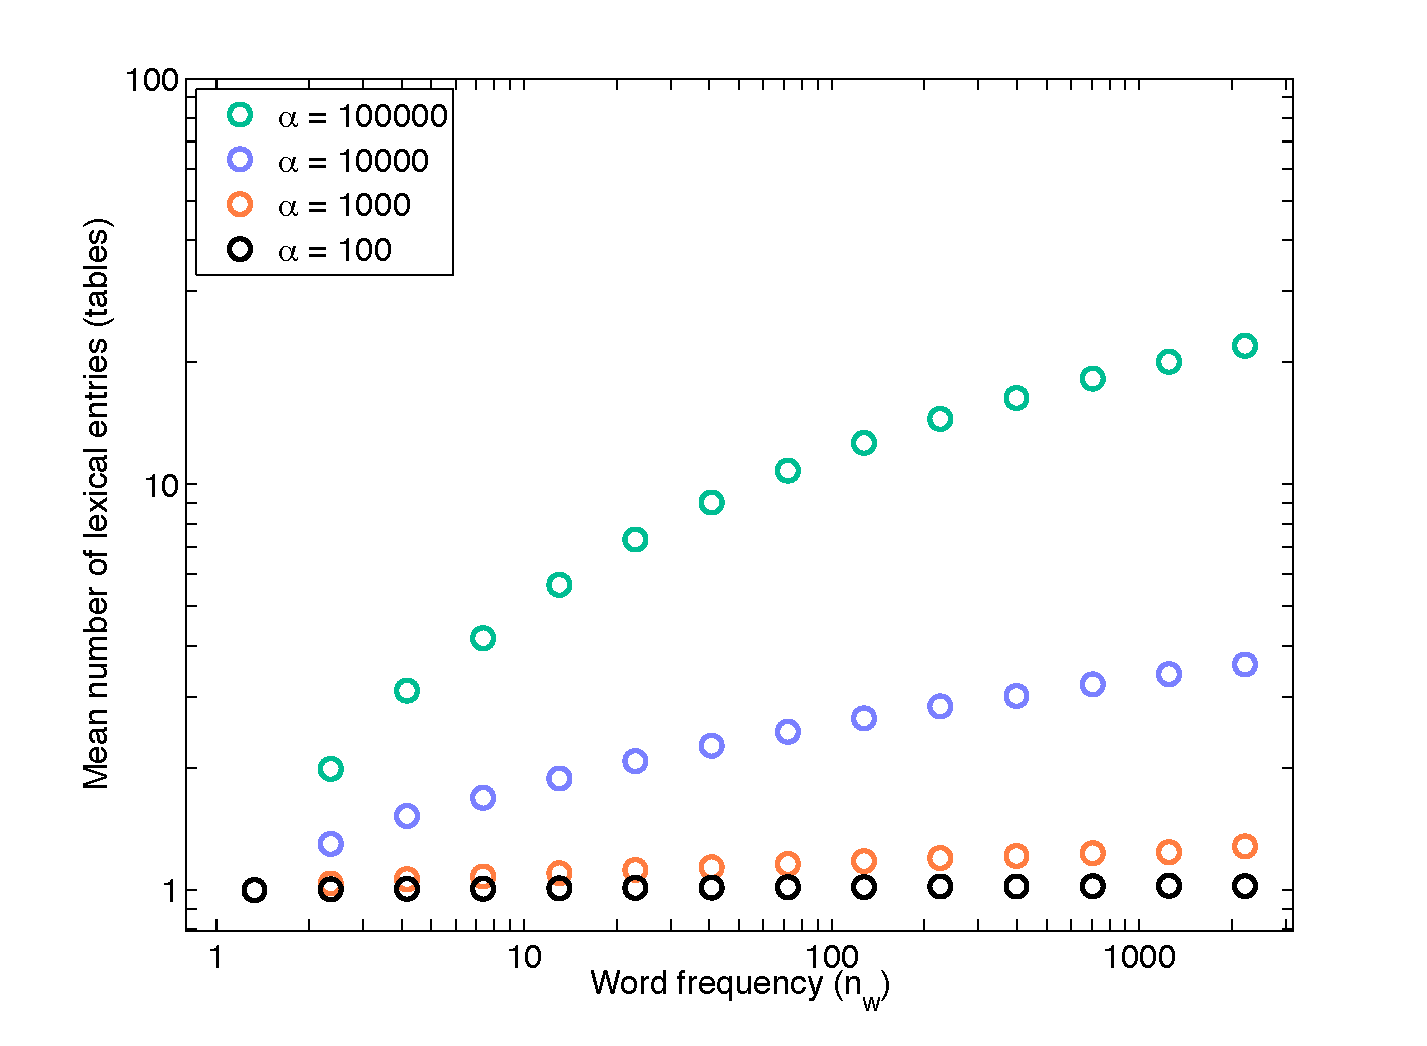
\includegraphics[scale=0.45]{code/plot0.pdf}}
\end{figure}
\end{frame}

\begin{frame}
\frametitle{DP performance}
\begin{figure}
{\centering 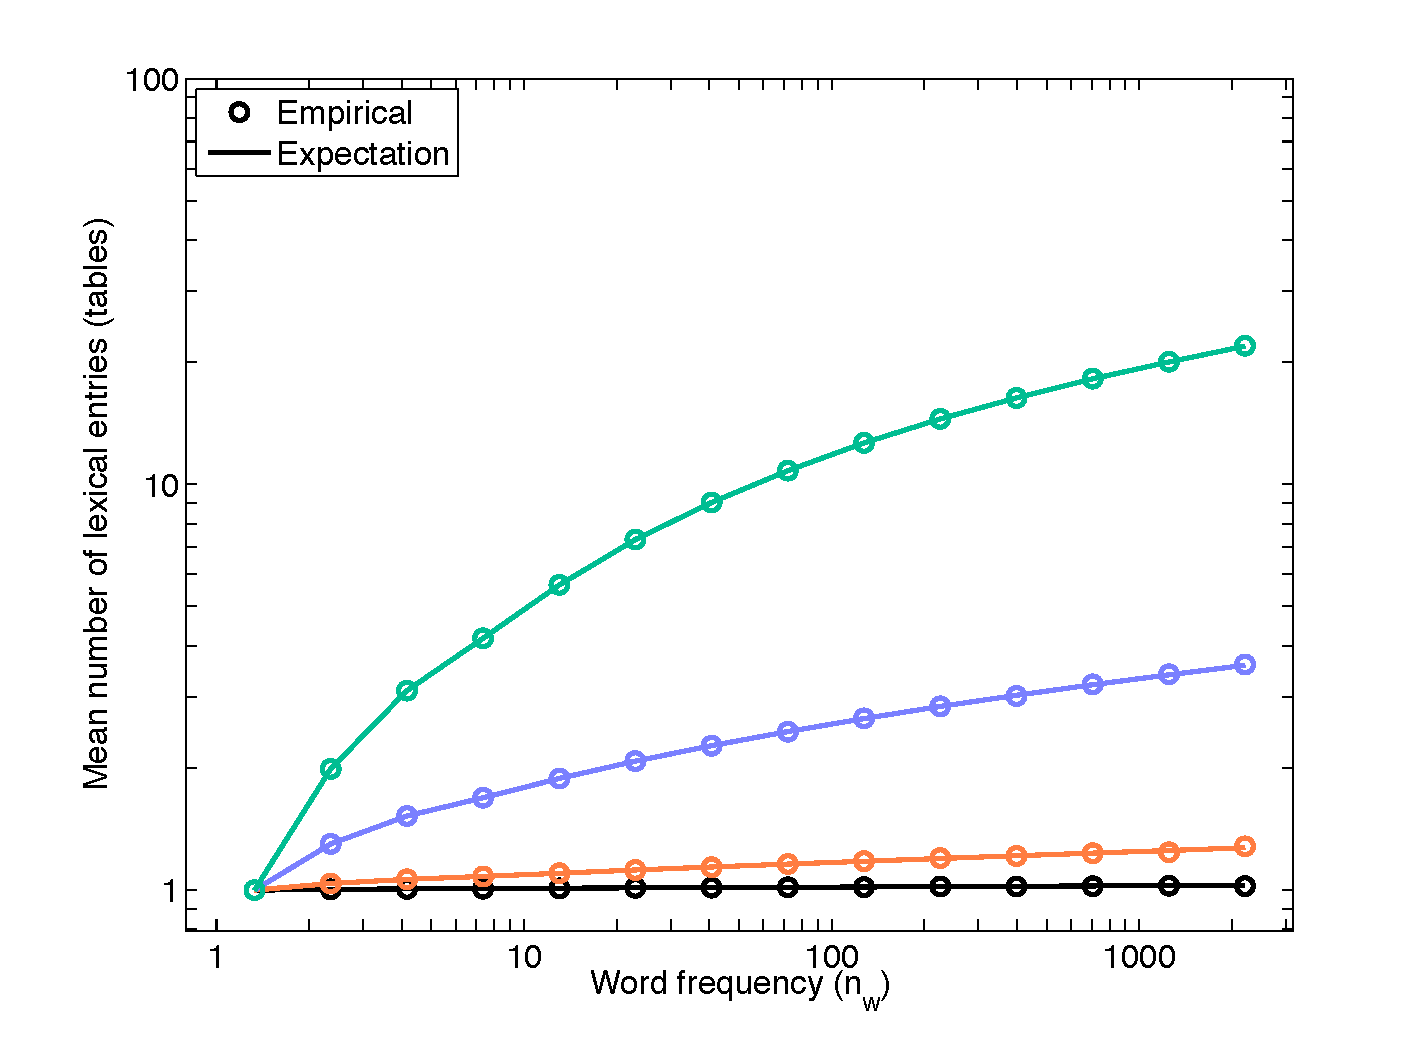
\includegraphics[scale=0.45]{code/plot1.pdf}}
\end{figure}
\end{frame}

\begin{frame}
\frametitle{DP performance}
\begin{figure}
{\centering 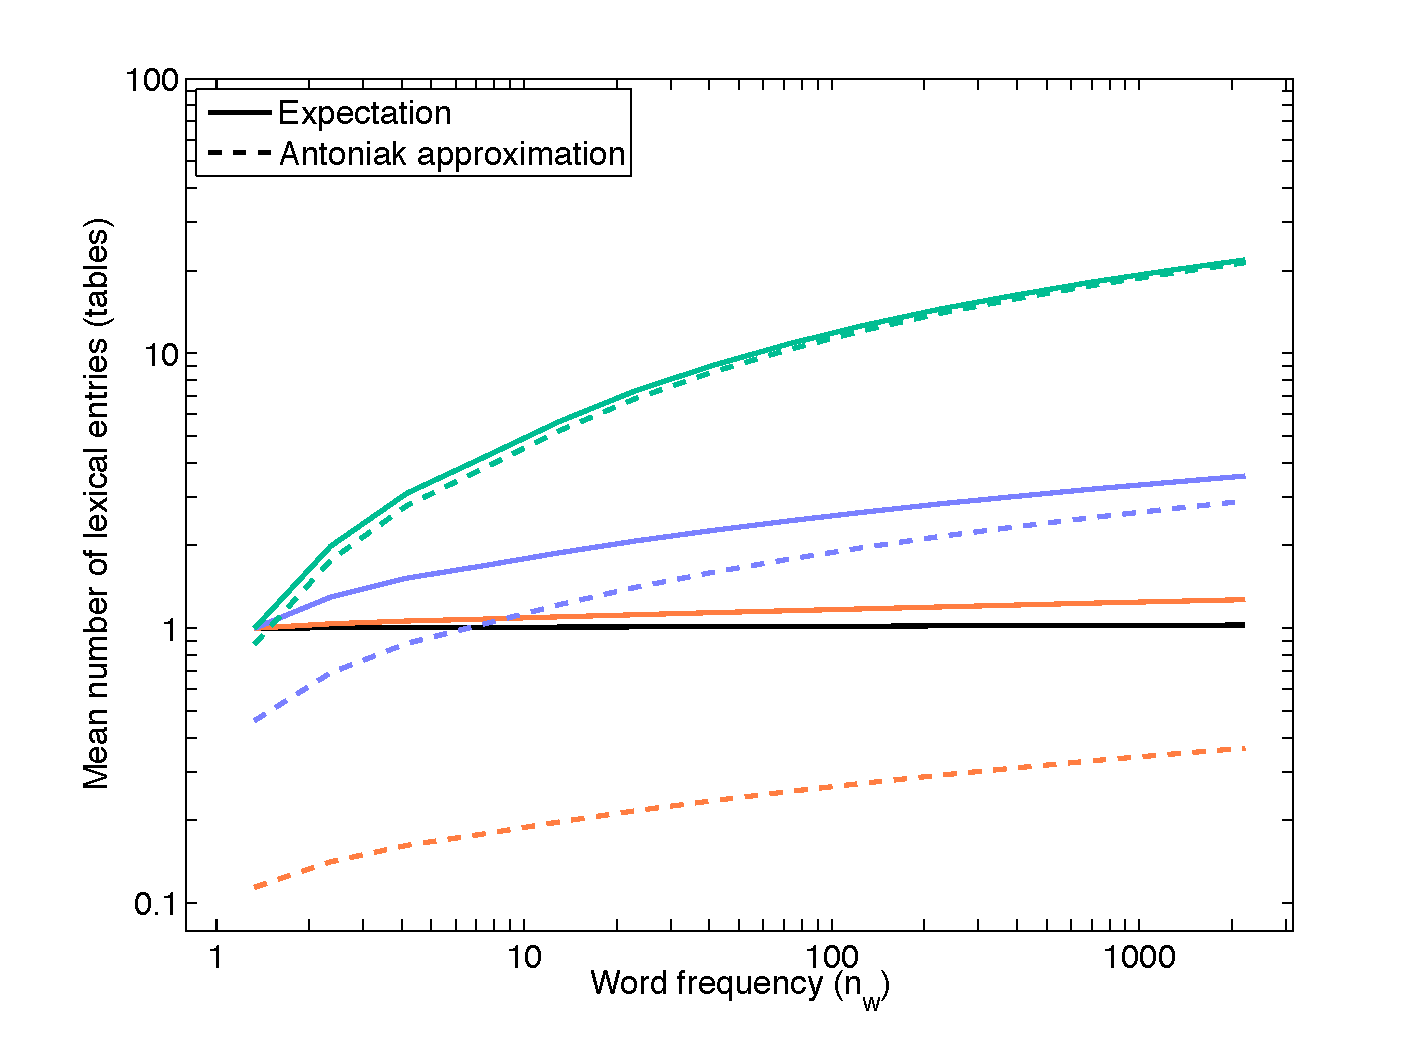
\includegraphics[scale=0.45]{code/plot2.pdf}}
\end{figure}
\end{frame}

\begin{frame}
\frametitle{HDP performance}
\begin{figure}
{\centering 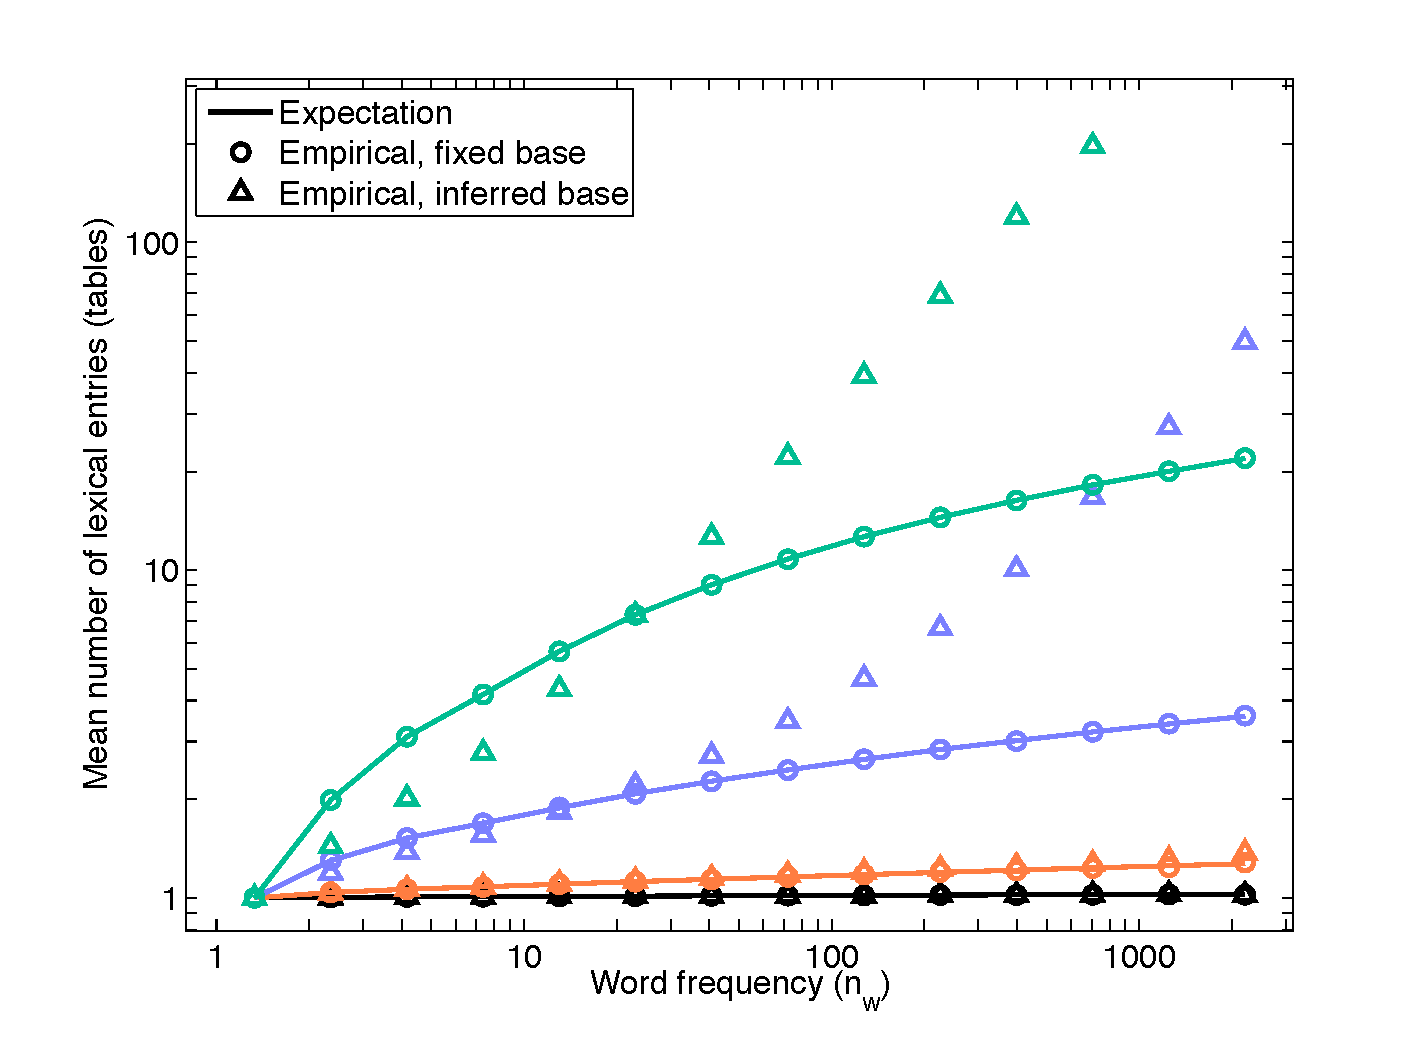
\includegraphics[scale=0.45]{code/plot3.pdf}}
\end{figure}
\end{frame}

\begin{frame}
\frametitle{Histogram Method}
\begin{unpacked_itemize}
  \item At this point we don't have a useful approximation of the expected table
    counts in a HDP model.
  \item However, we can describe a more compact representation for the state of the restaurant that doesn't require explicit table tracking.
  \item Instead we maintain a histogram for each dish $w_i$ of the frequency of a table having a particular number of customers.
\end{unpacked_itemize}
\end{frame}

\begin{frame}[t]
\frametitle{Histogram Method}
\begin{center}
  \only<1>{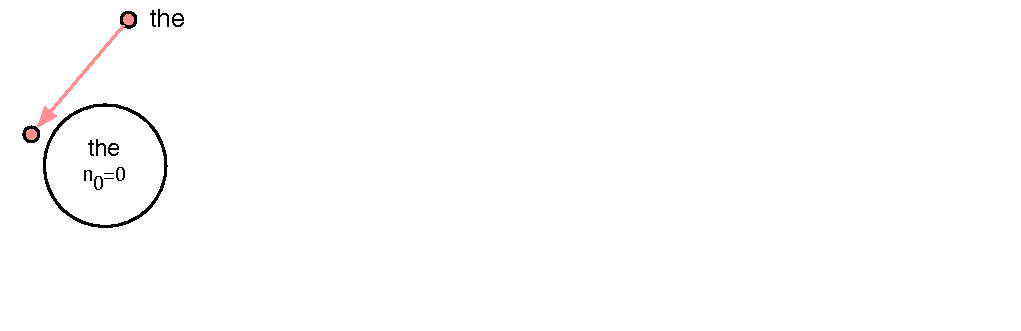
\includegraphics[scale=0.7]{tables0.pdf}}
  \only<2>{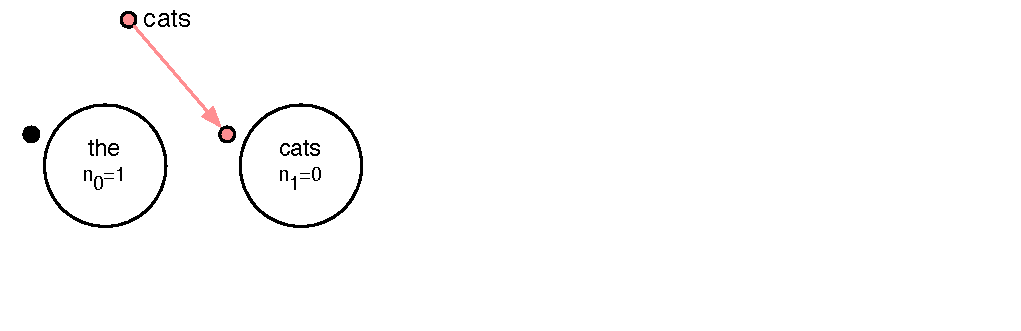
\includegraphics[scale=0.7]{tables1.pdf}}
  \only<3>{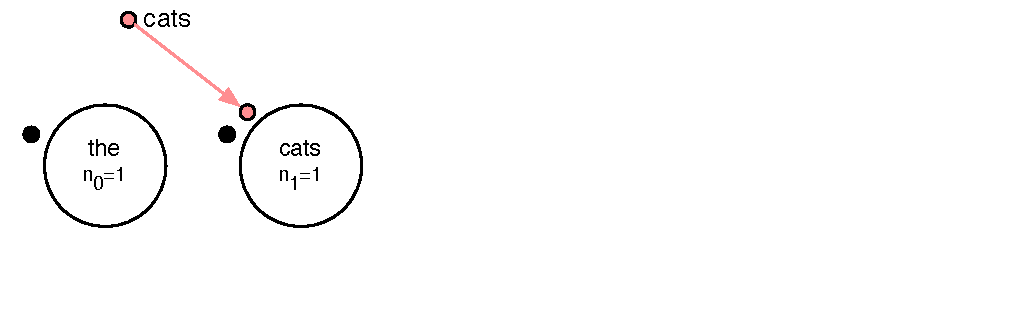
\includegraphics[scale=0.7]{tables2.pdf}}
  \only<4>{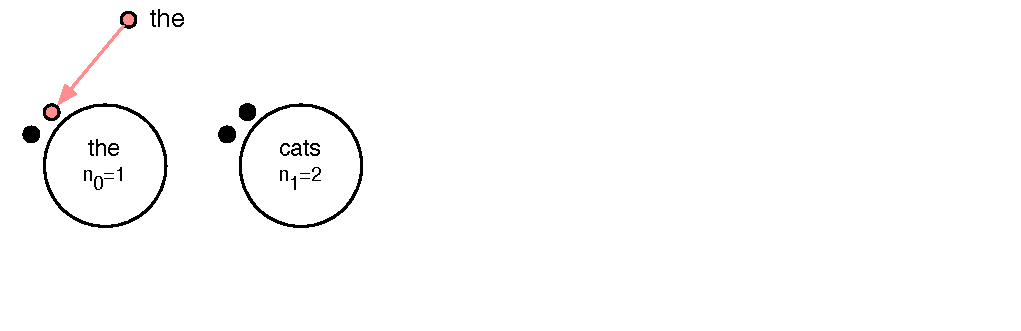
\includegraphics[scale=0.7]{tables3.pdf}}
  \only<5>{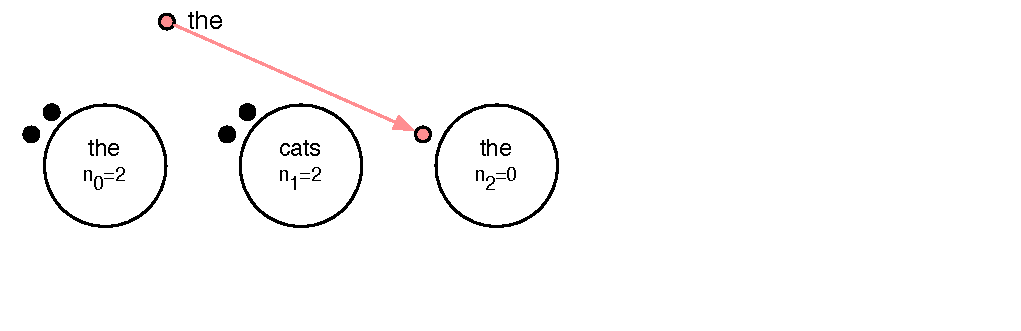
\includegraphics[scale=0.7]{tables4.pdf}}
  \only<6>{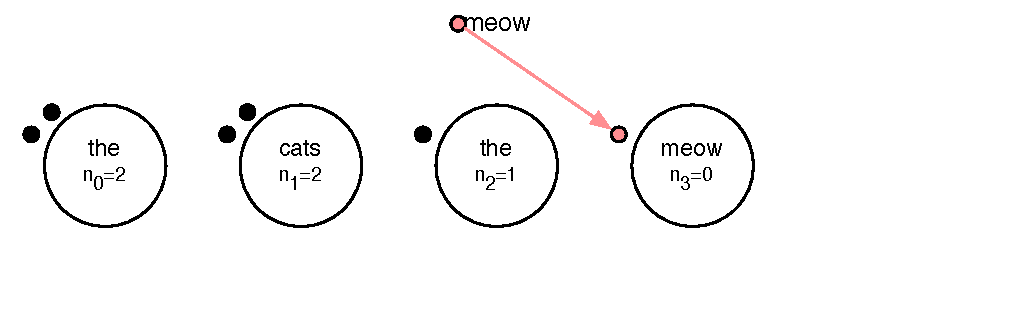
\includegraphics[scale=0.7]{tables5.pdf}}
  \only<7>{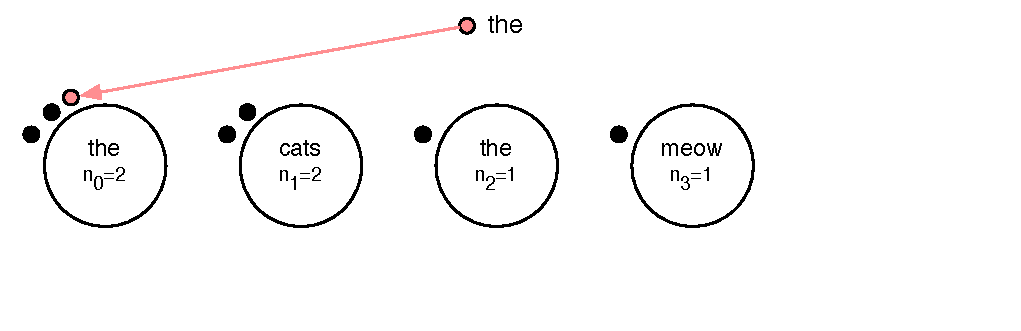
\includegraphics[scale=0.7]{tables7.pdf}}
  \only<8>{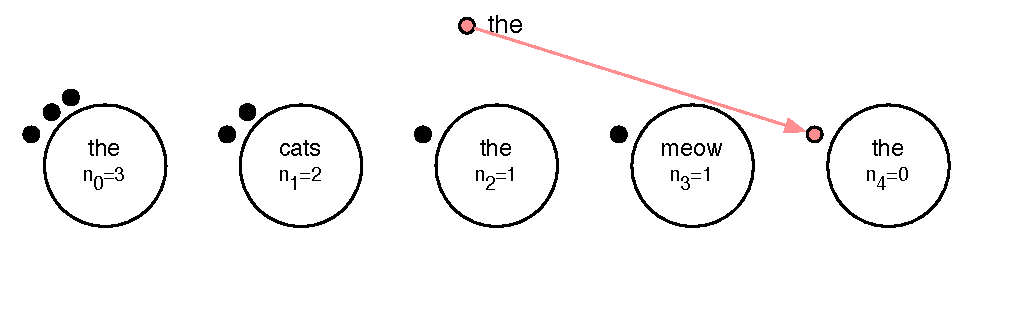
\includegraphics[scale=0.7]{tables9.pdf}}
\end{center}
\vspace{-2.5cm}
\only<6->{\vspace{0.47cm}}
\begin{center}
  \only<1>{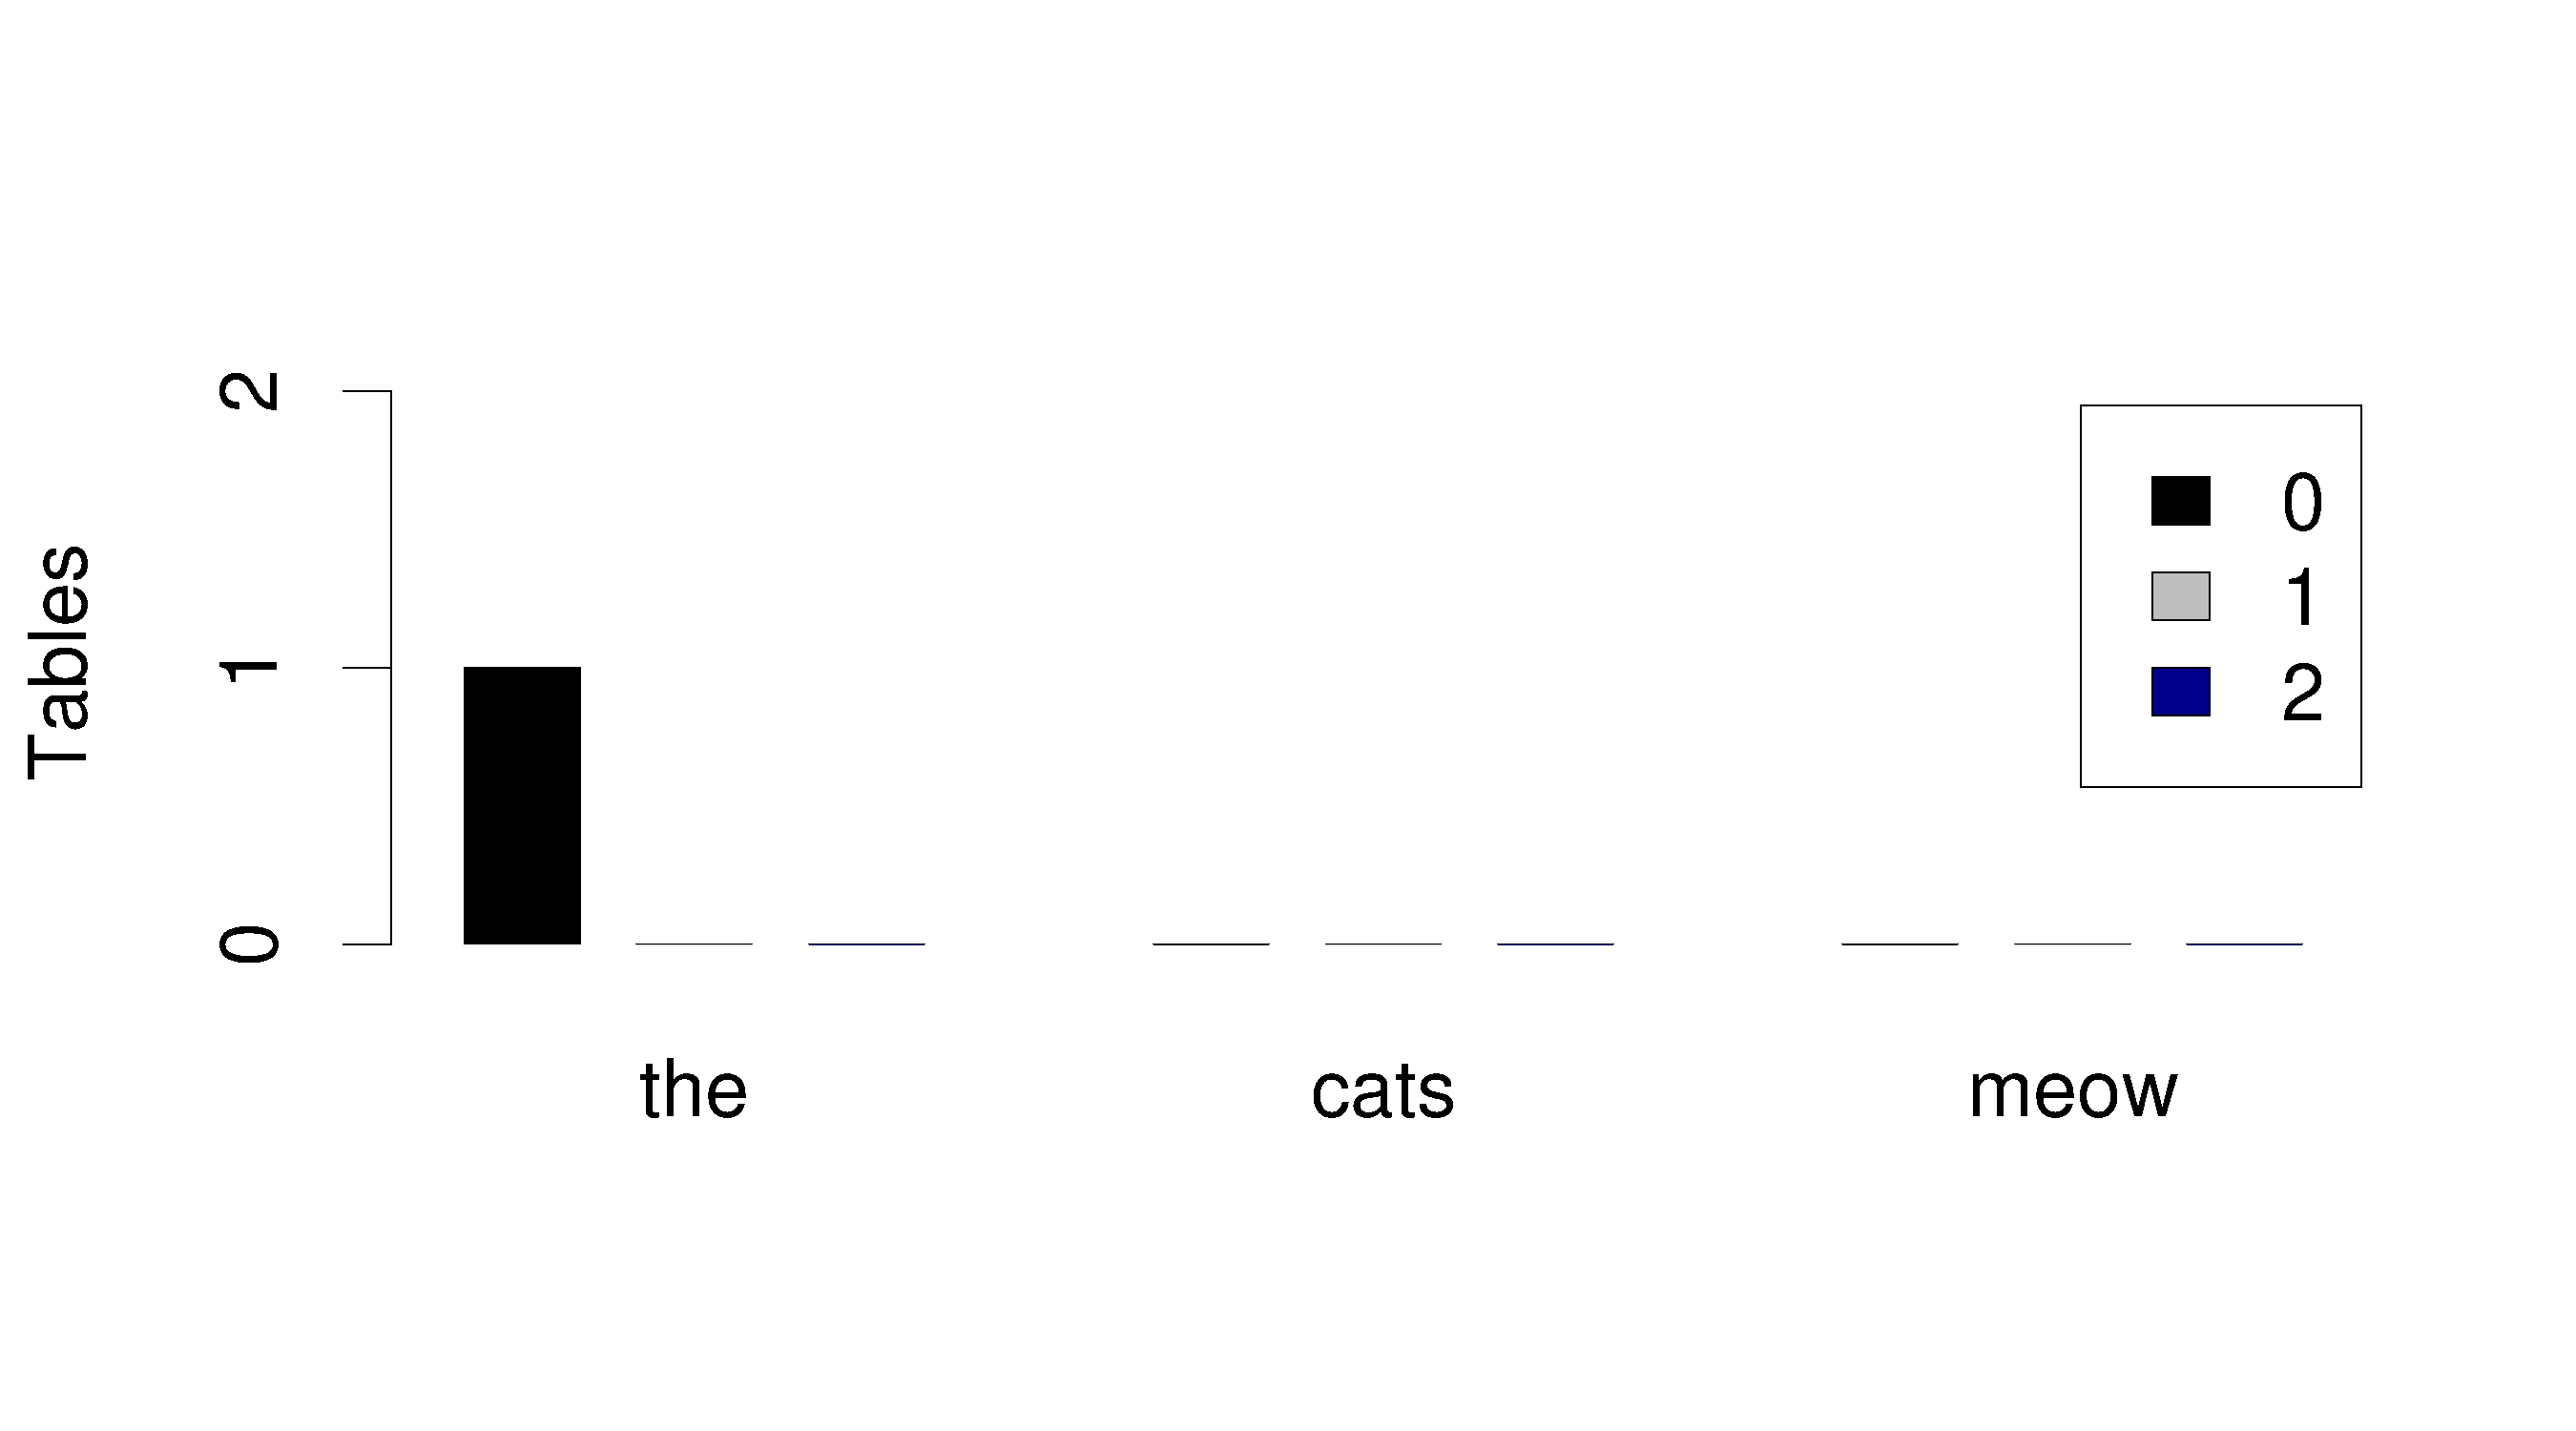
\includegraphics[scale=0.2]{histogram_1.pdf}\hspace{-0.6cm}}
  \only<2>{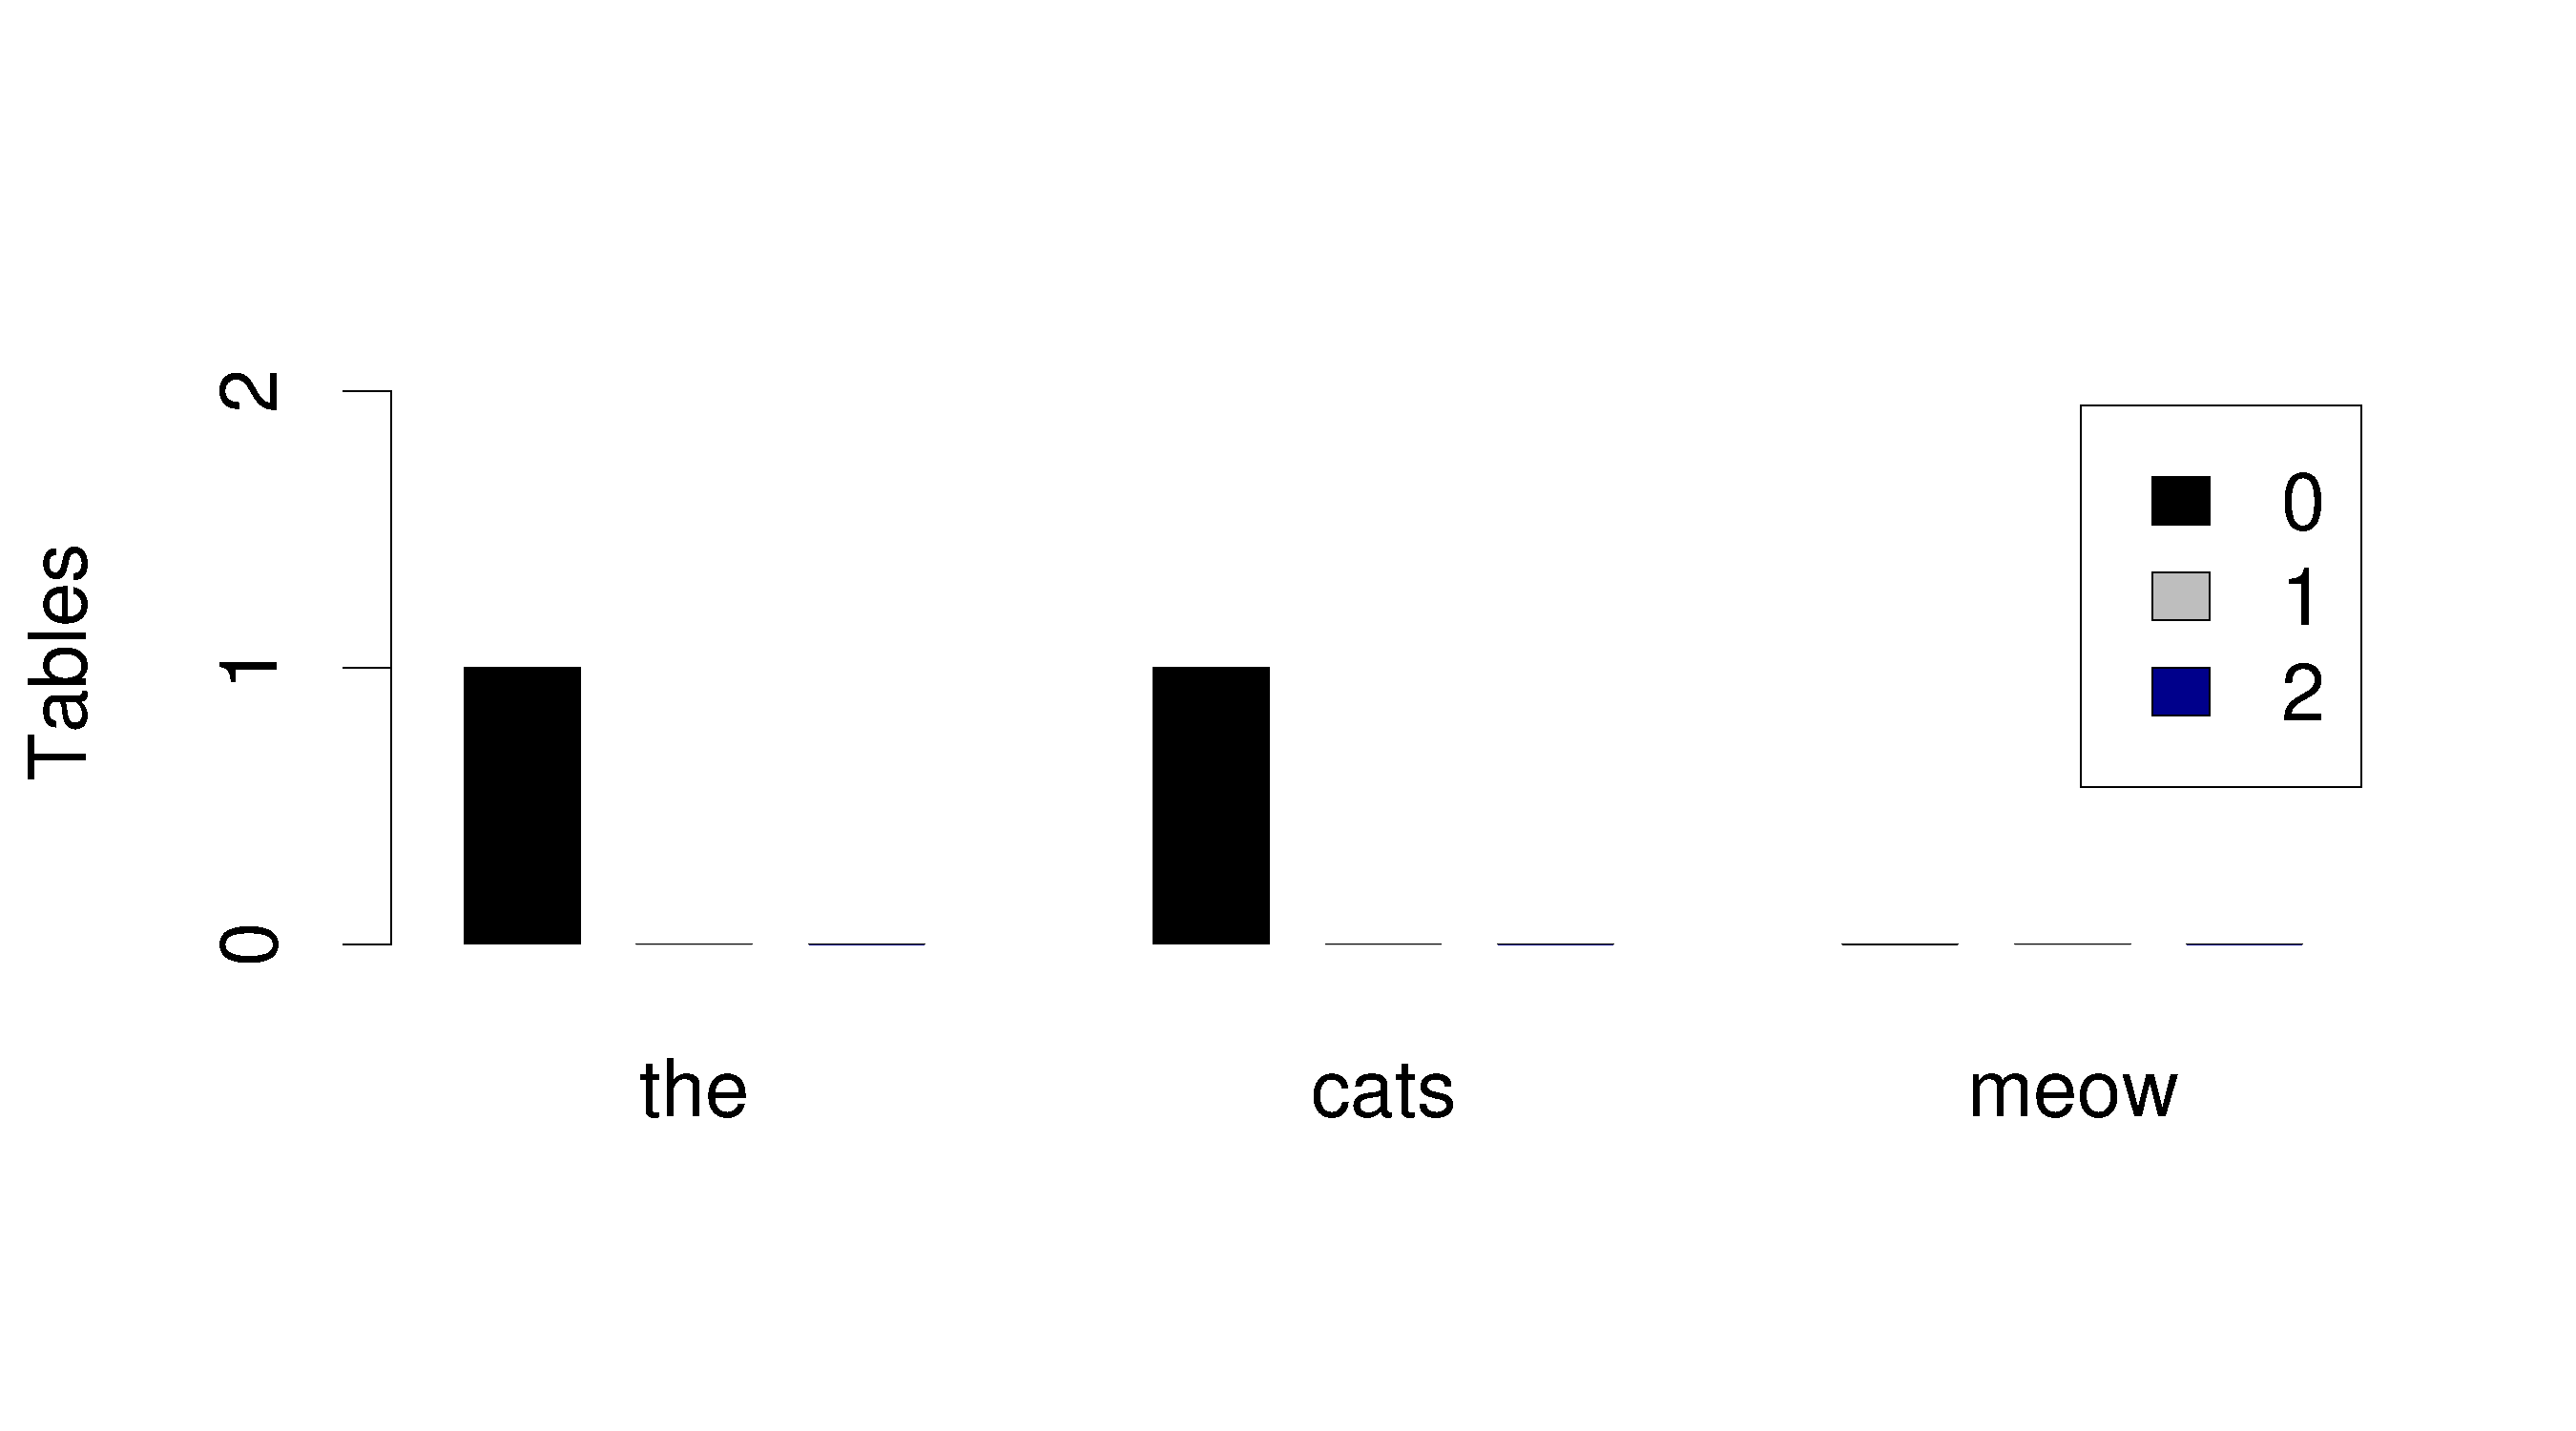
\includegraphics[scale=0.2]{histogram_2.pdf}\hspace{-0.5cm}}
  \only<3>{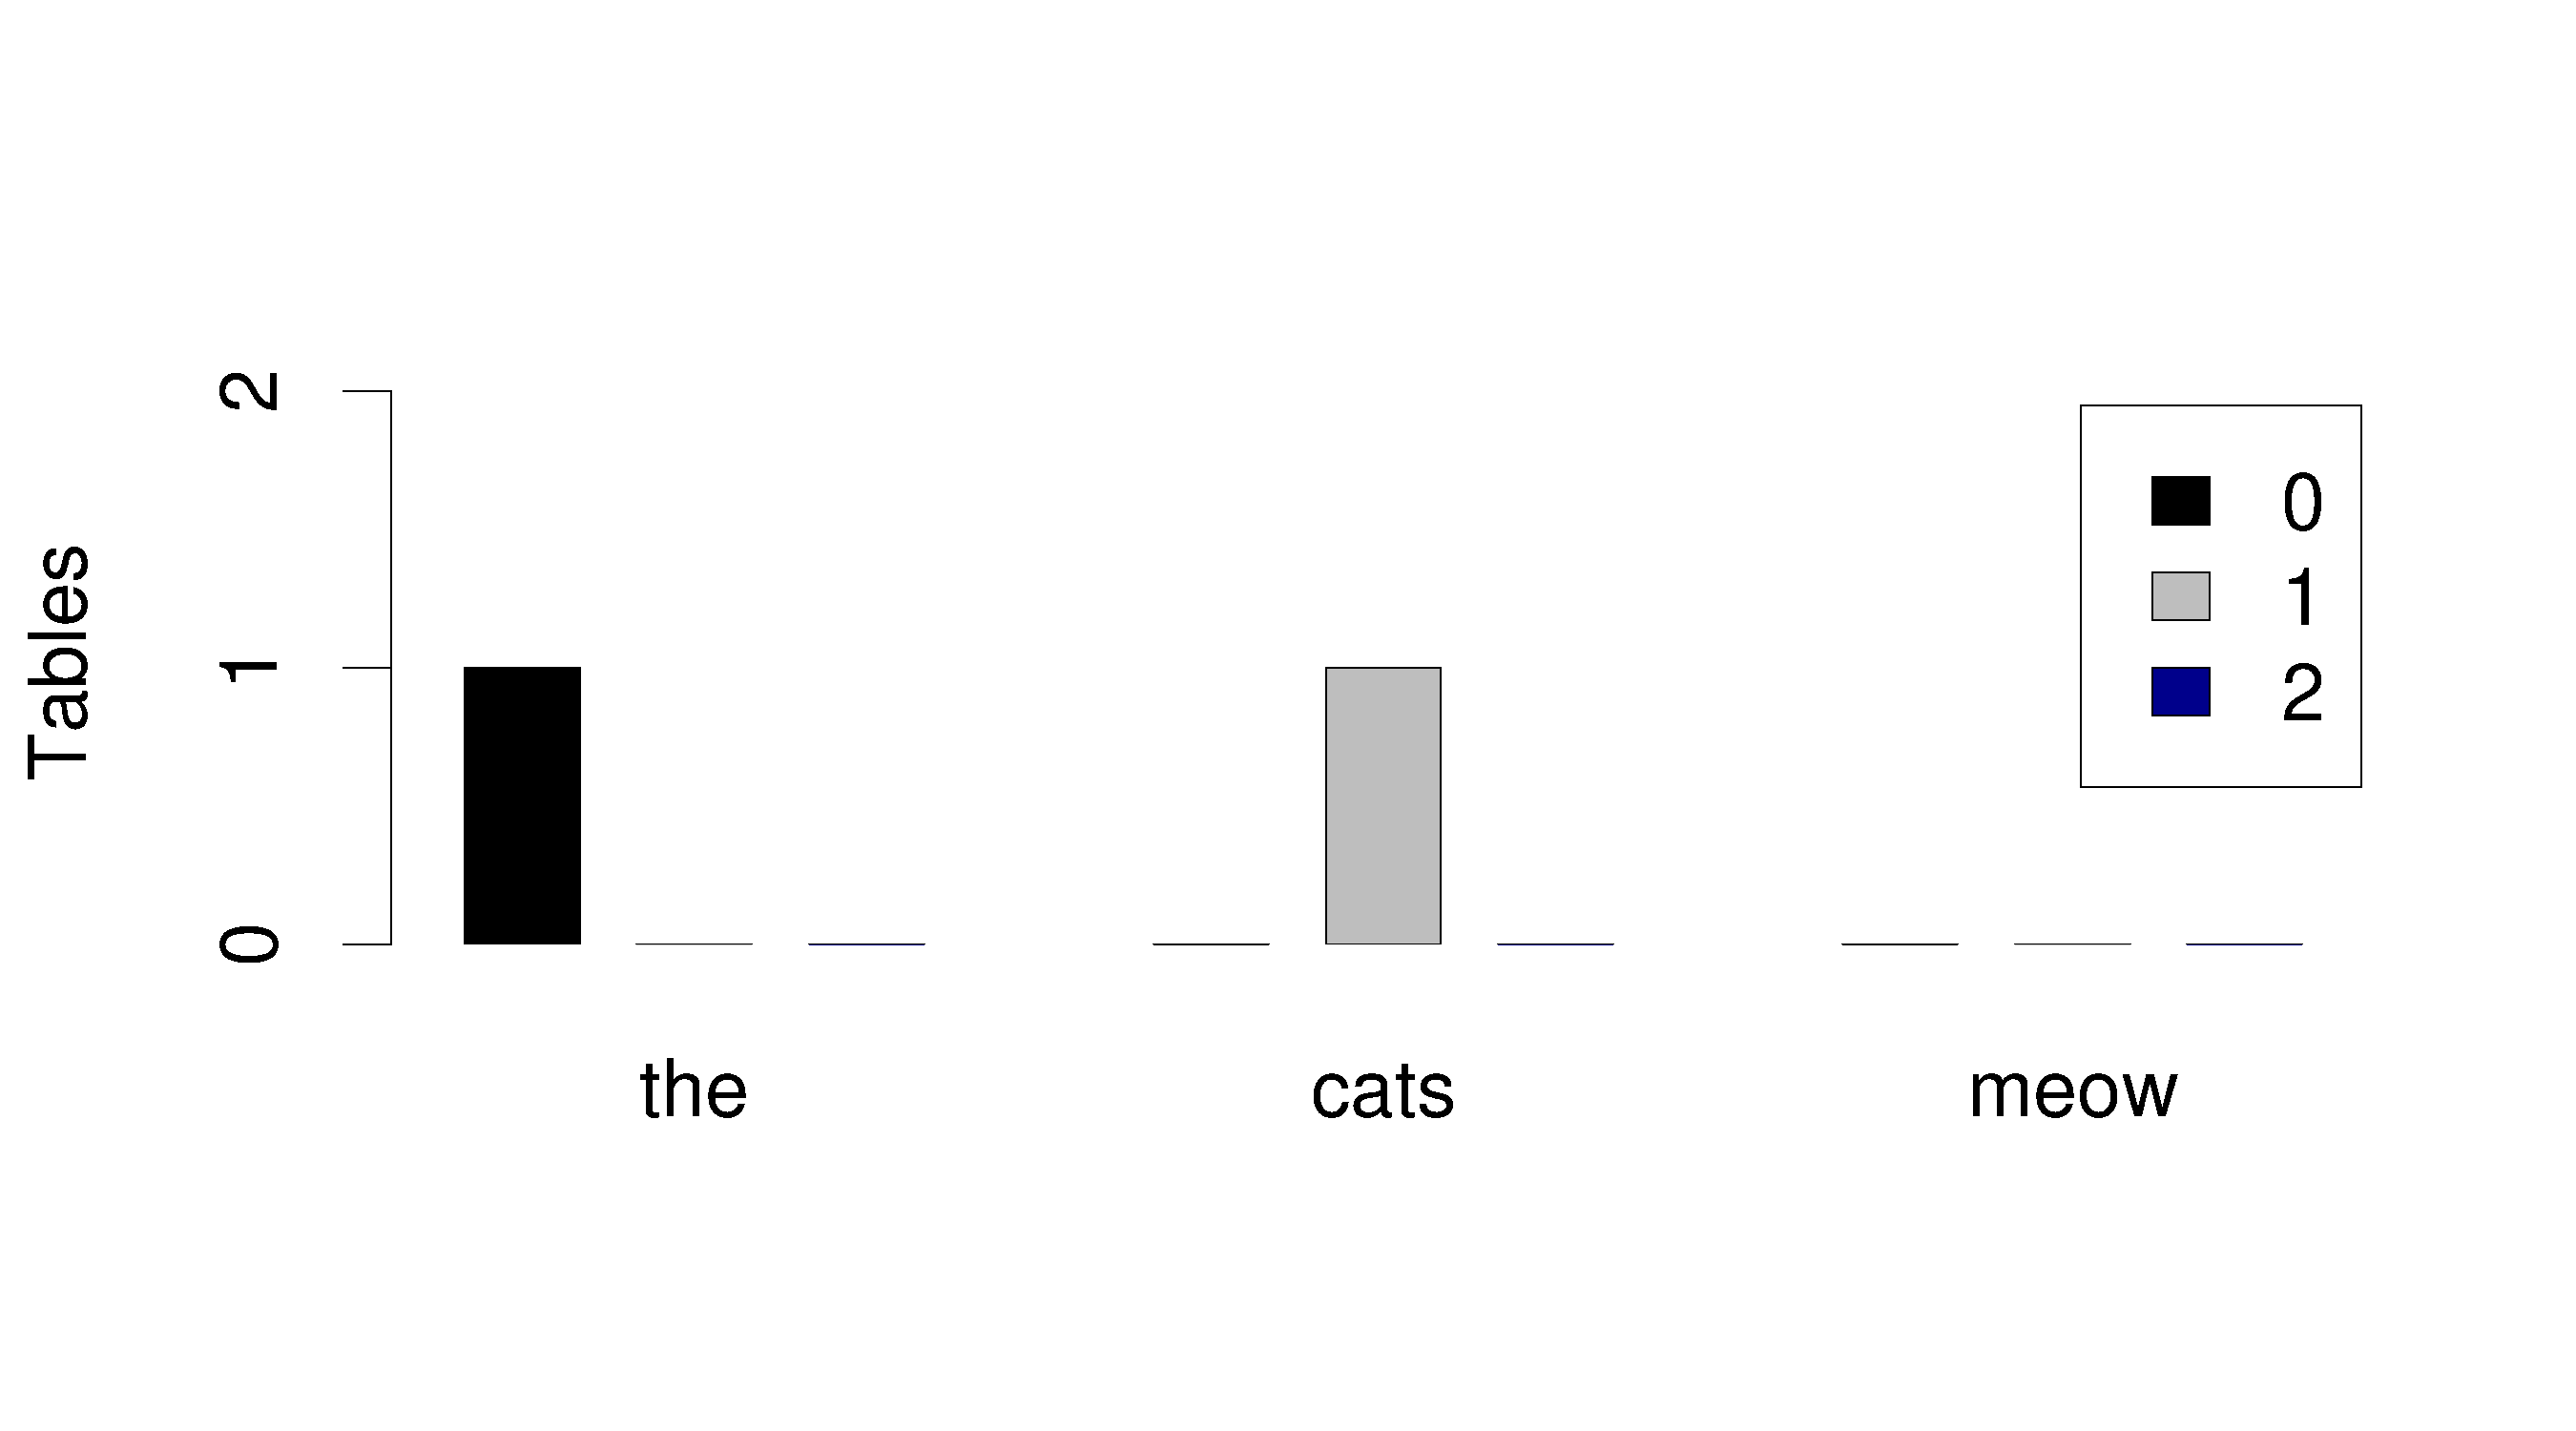
\includegraphics[scale=0.2]{histogram_3.pdf}\hspace{-0.4cm}}
  \only<4>{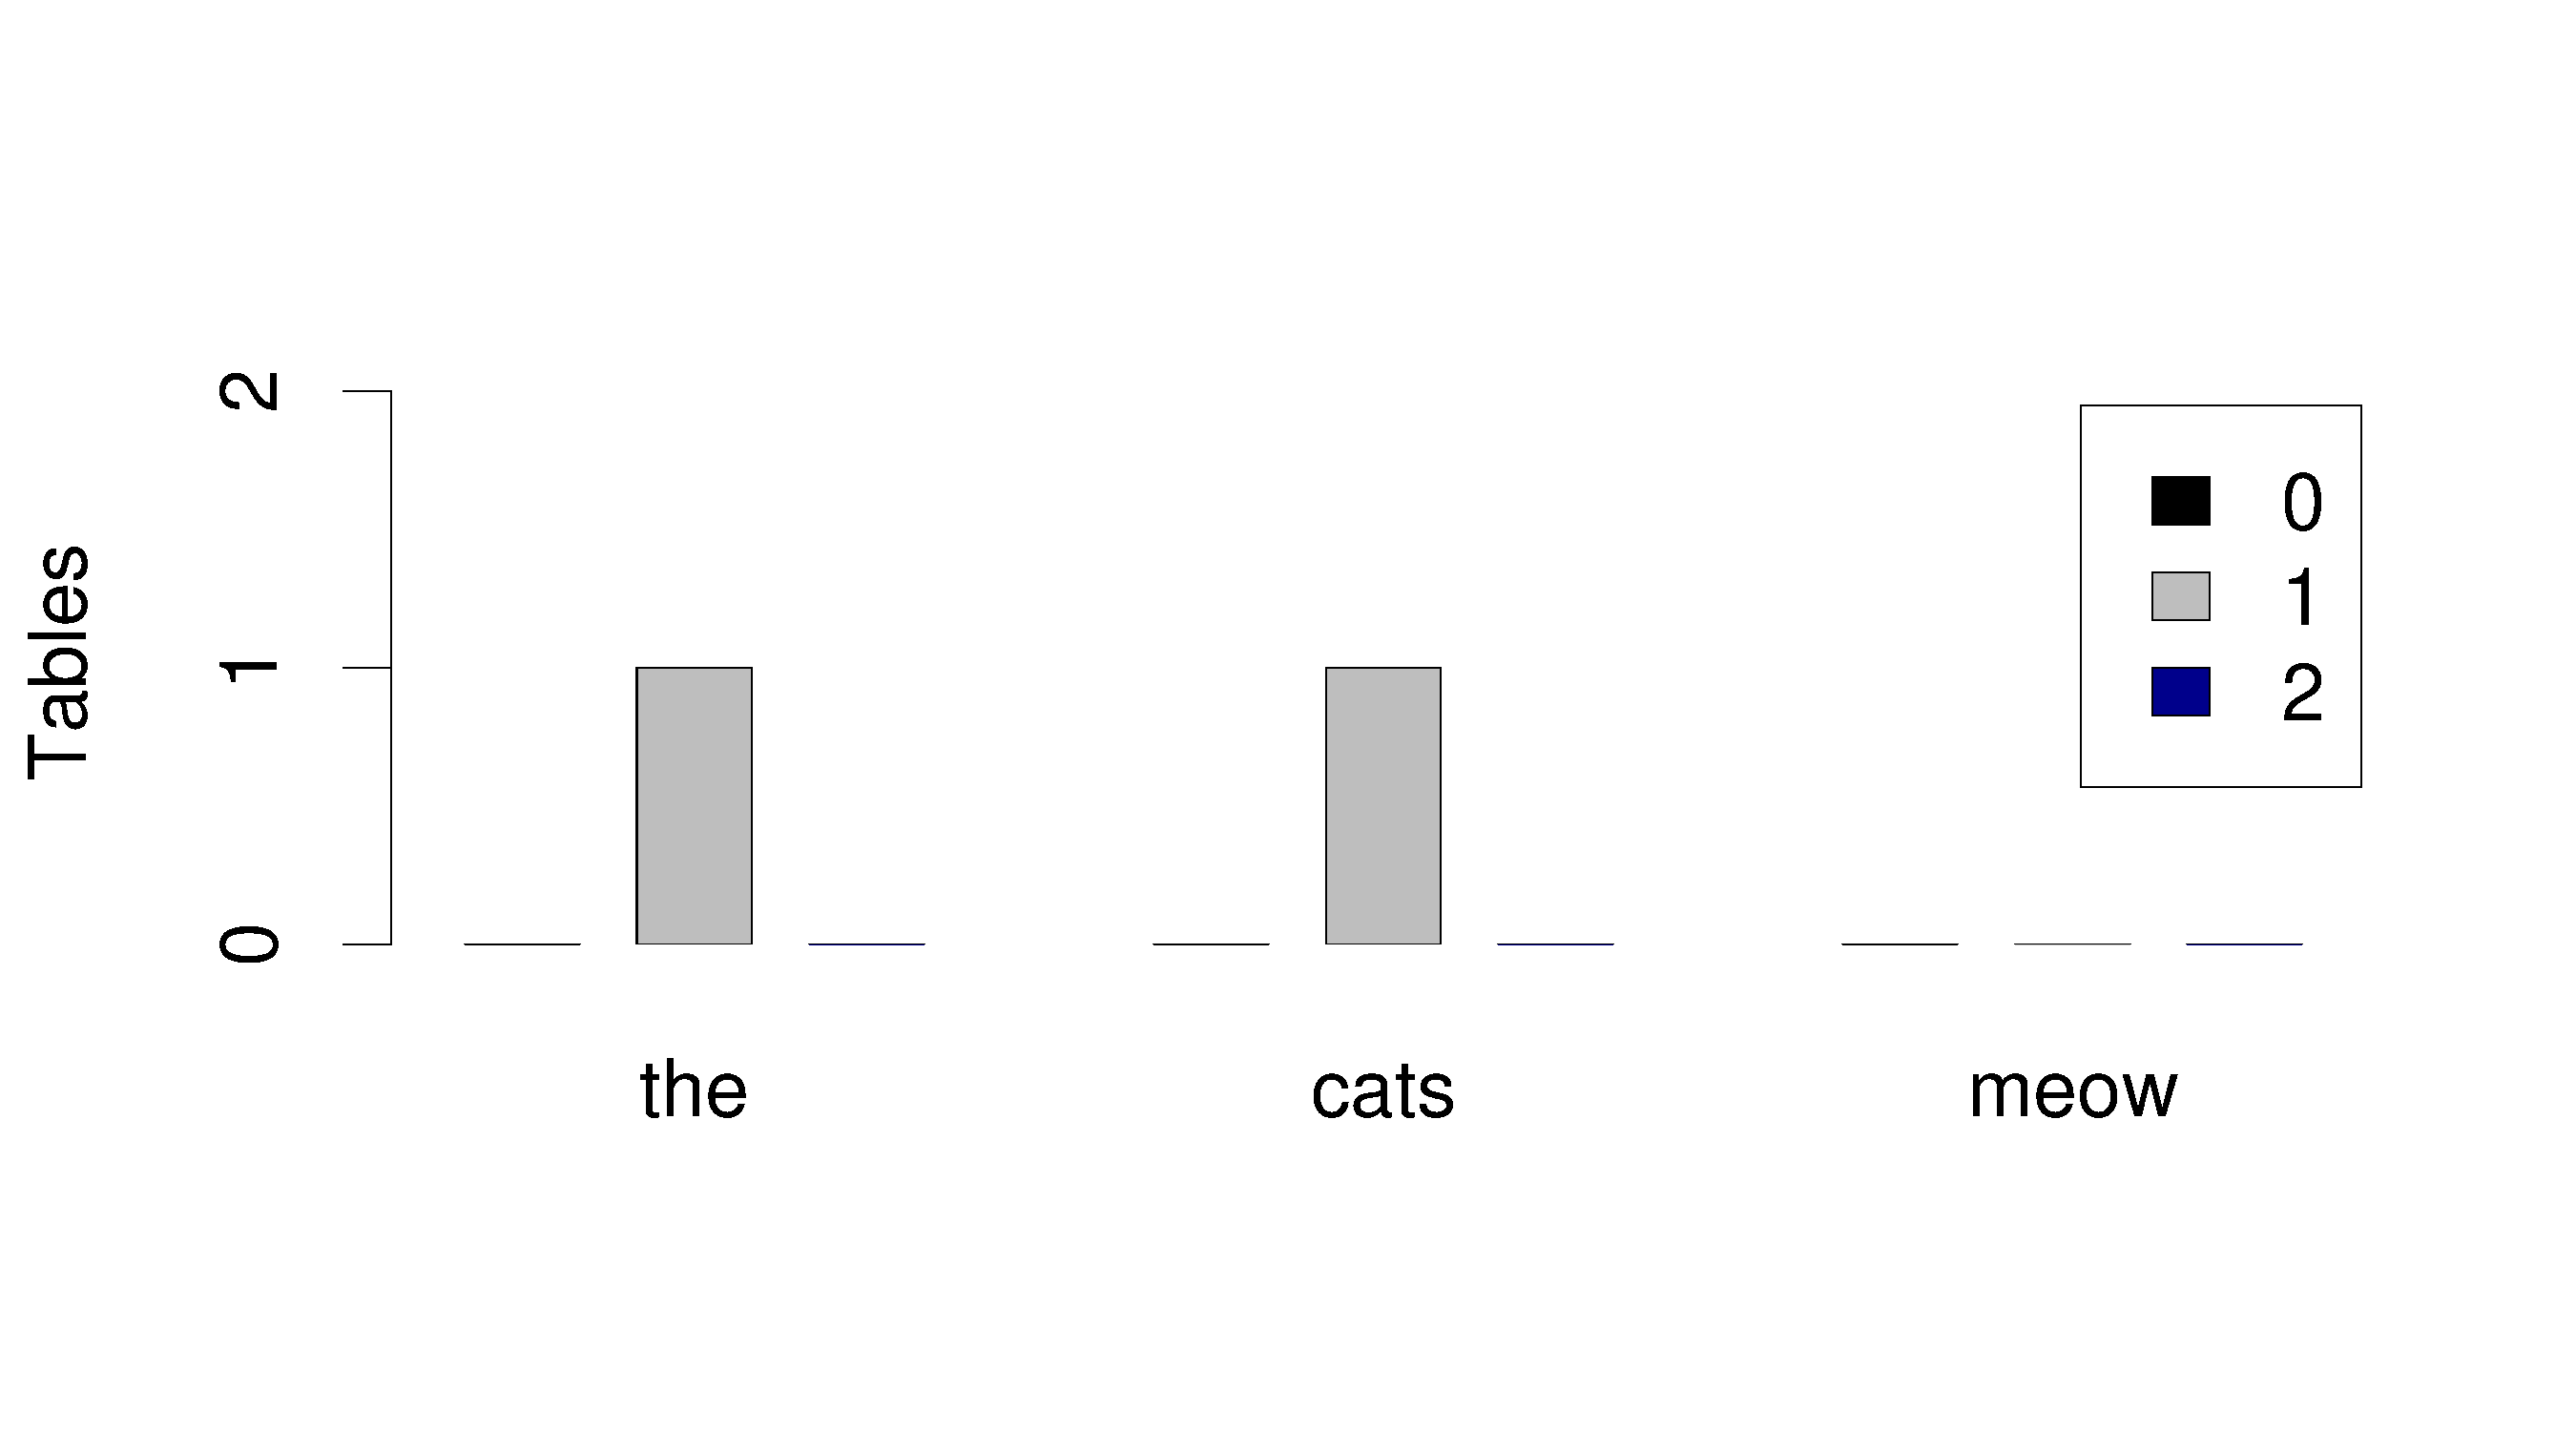
\includegraphics[scale=0.2]{histogram_4.pdf}\hspace{-0.3cm}}
  \only<5>{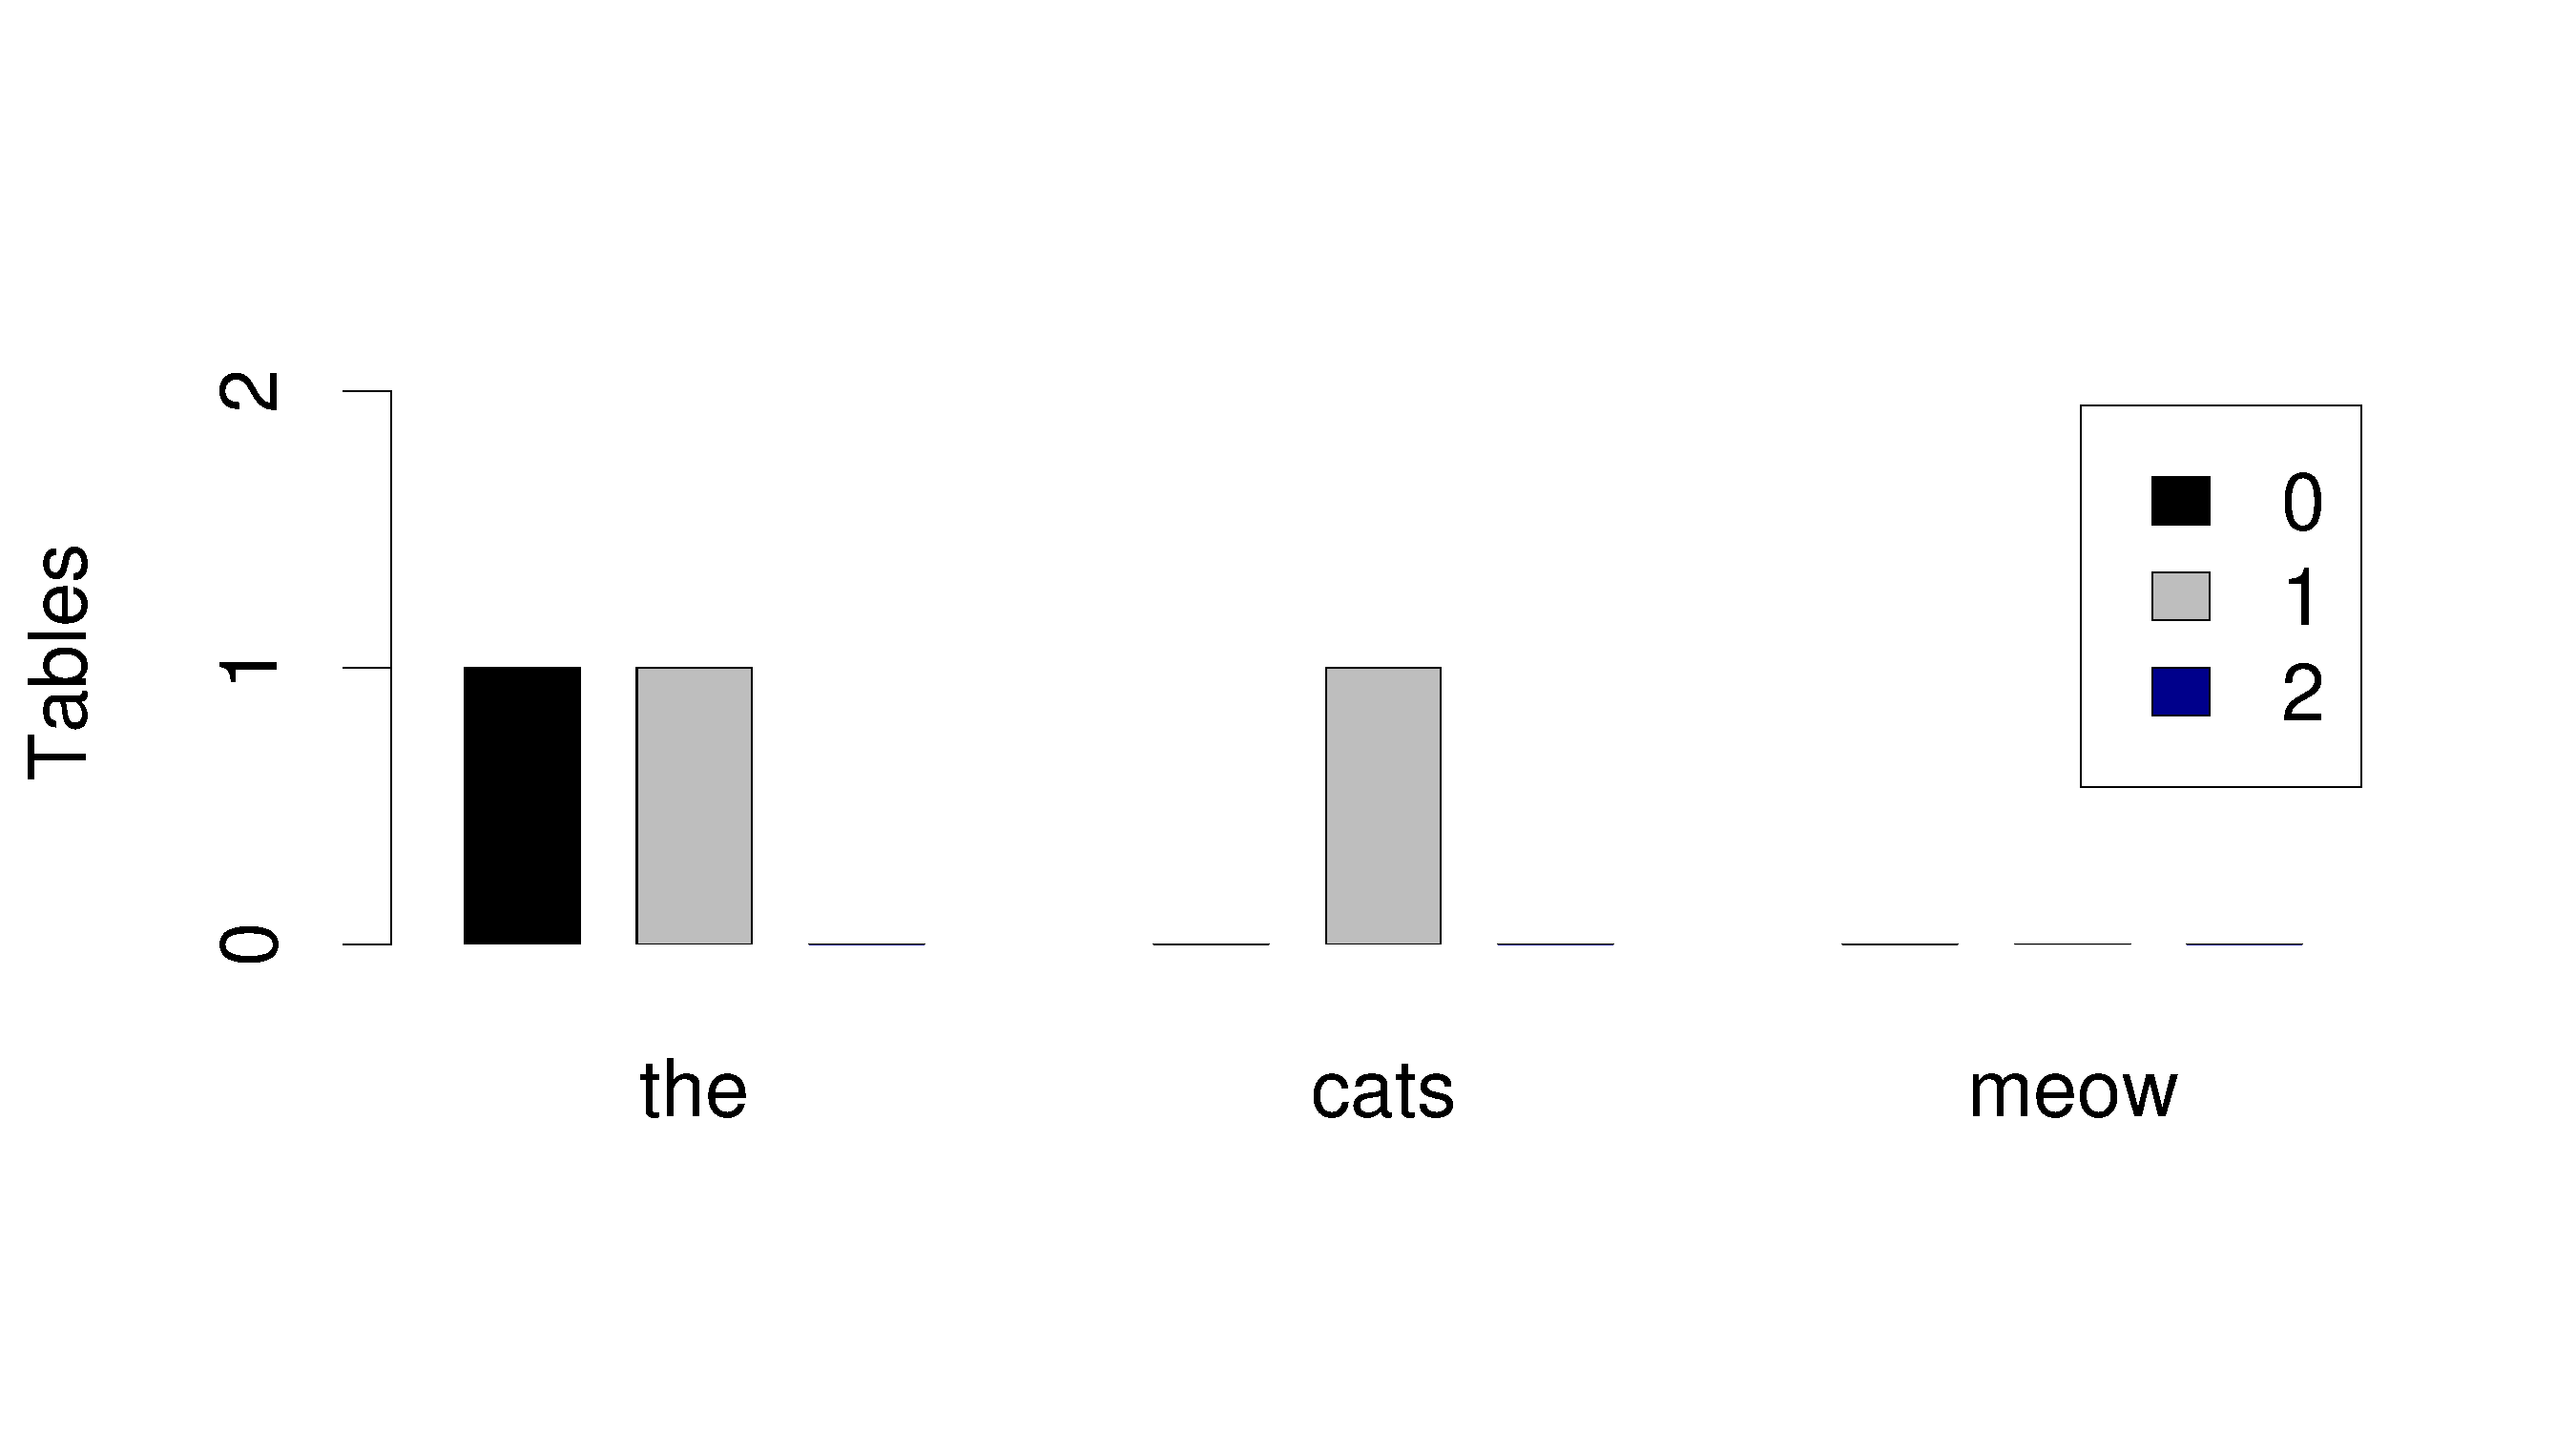
\includegraphics[scale=0.2]{histogram_5.pdf}\hspace{-0.2cm}}
  \only<6>{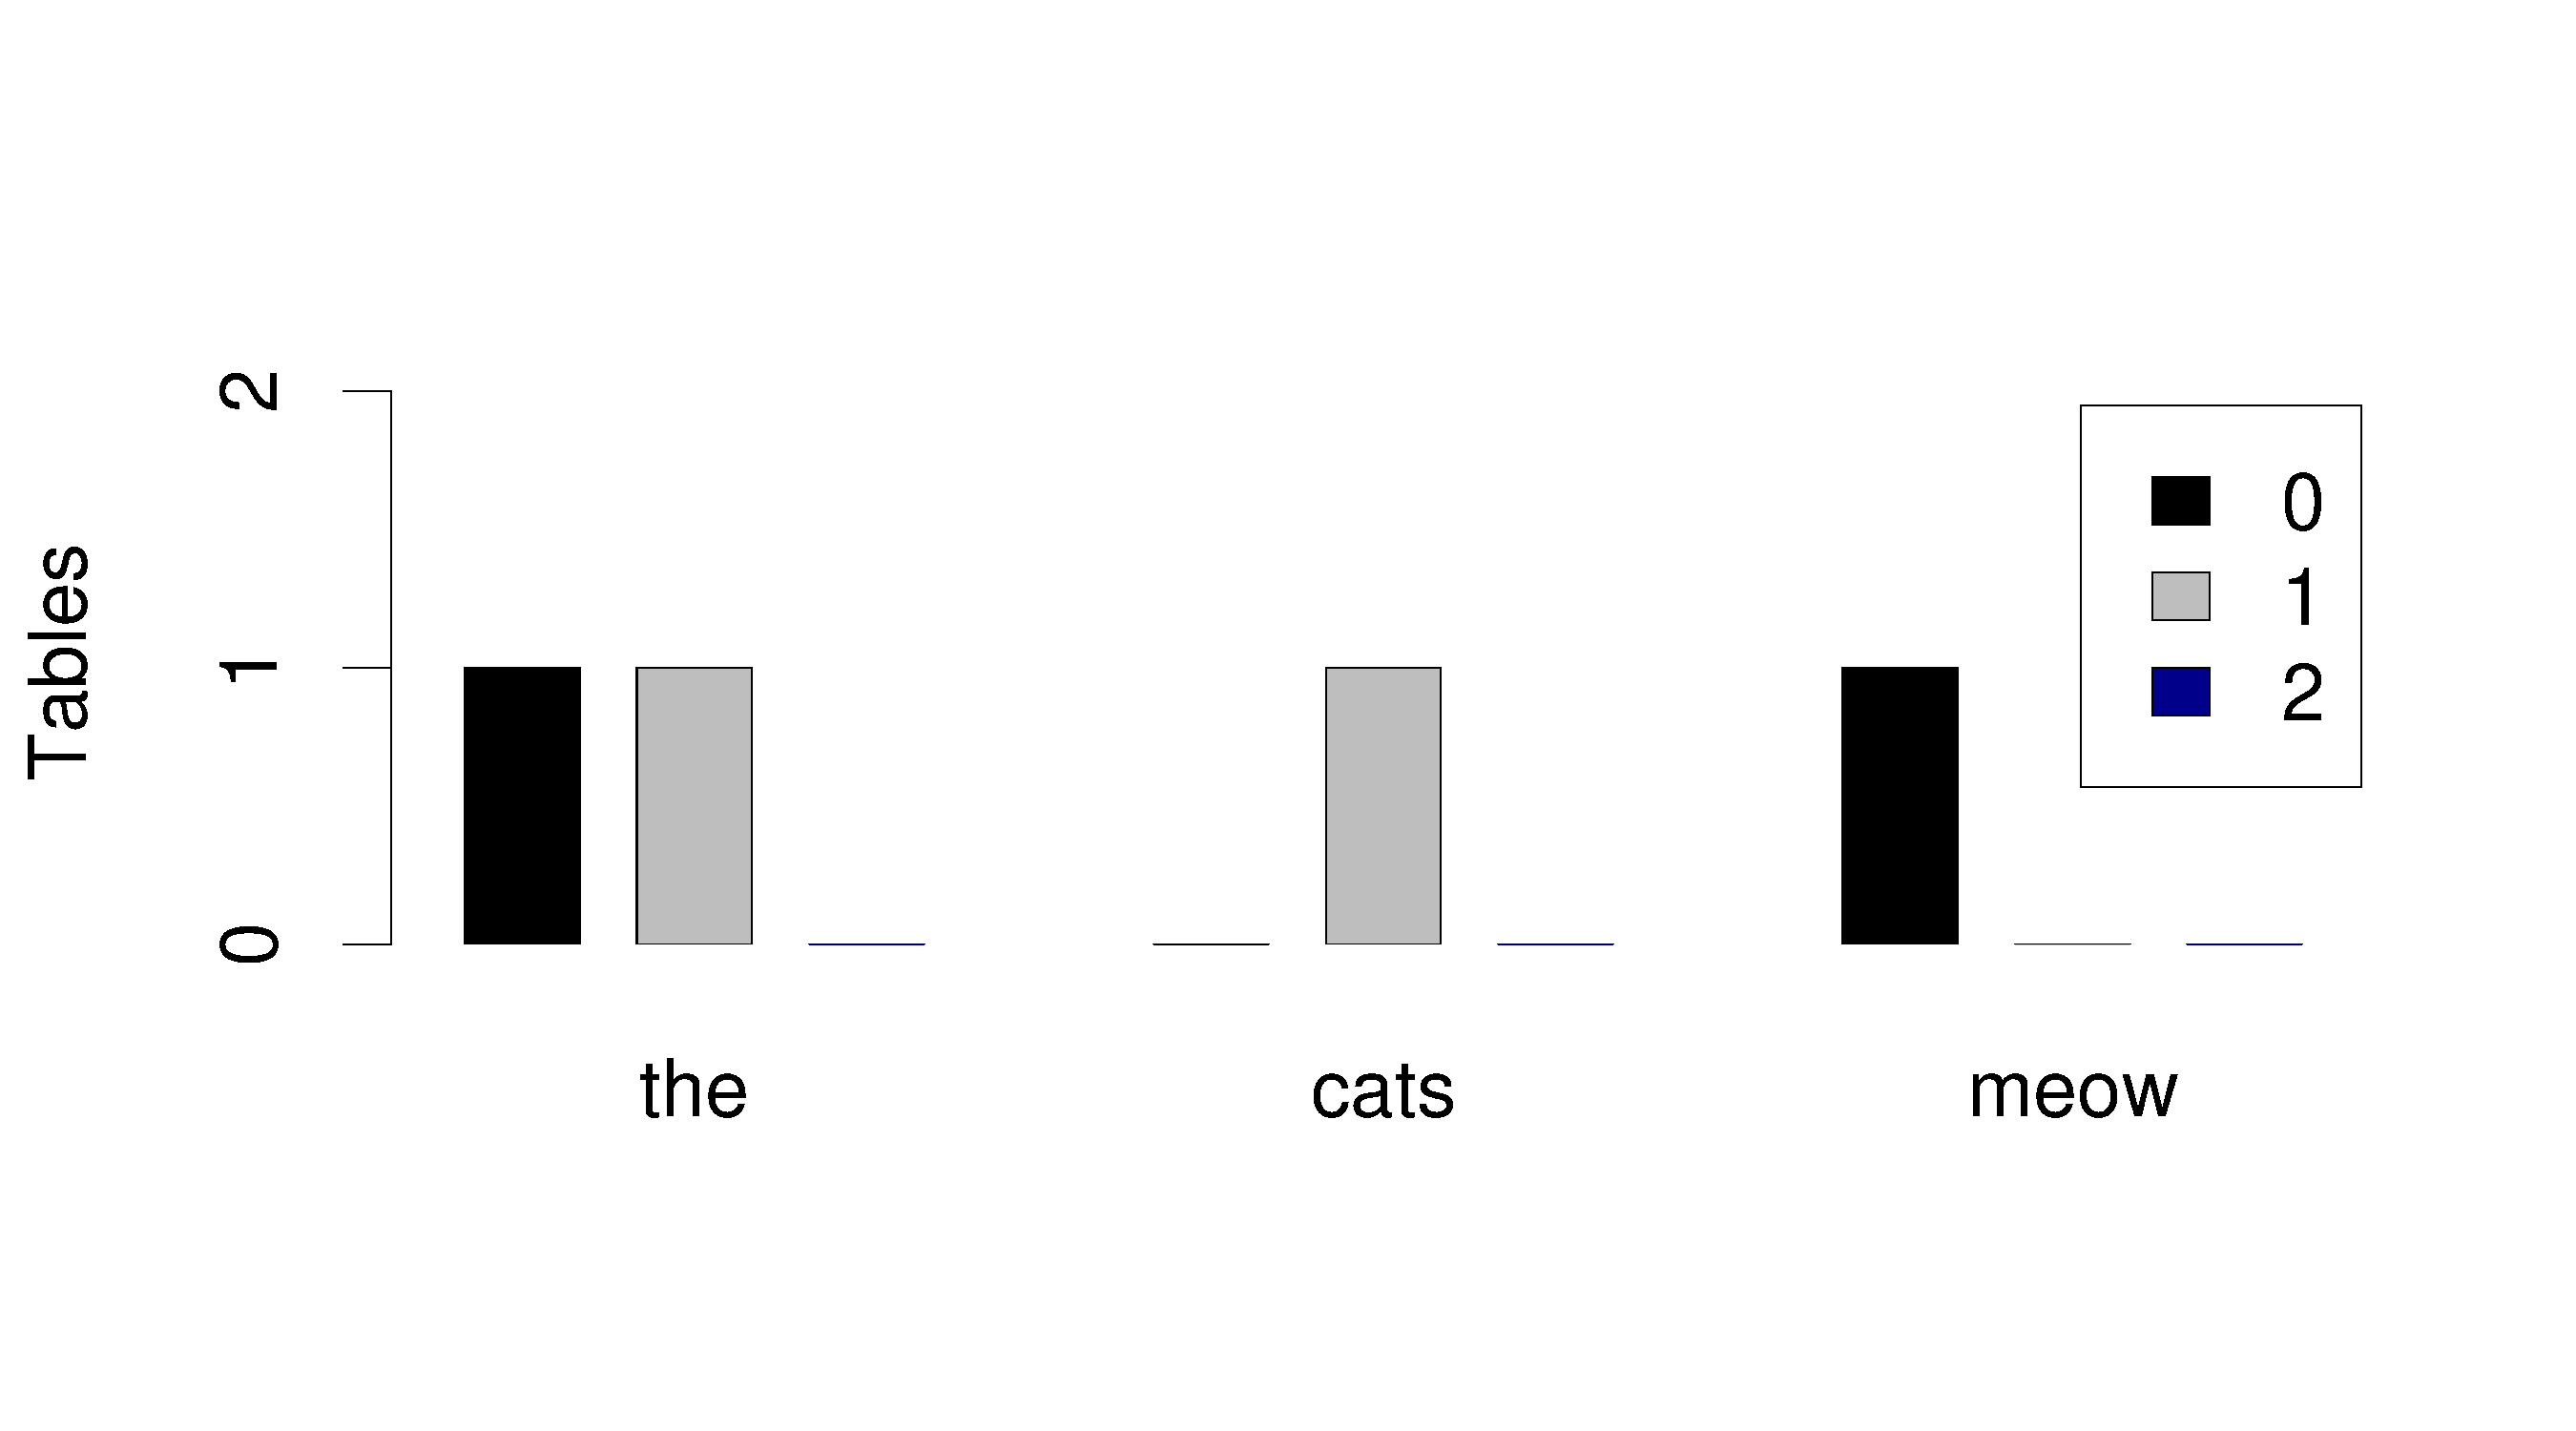
\includegraphics[scale=0.2]{histogram_6.pdf}}
  \only<7>{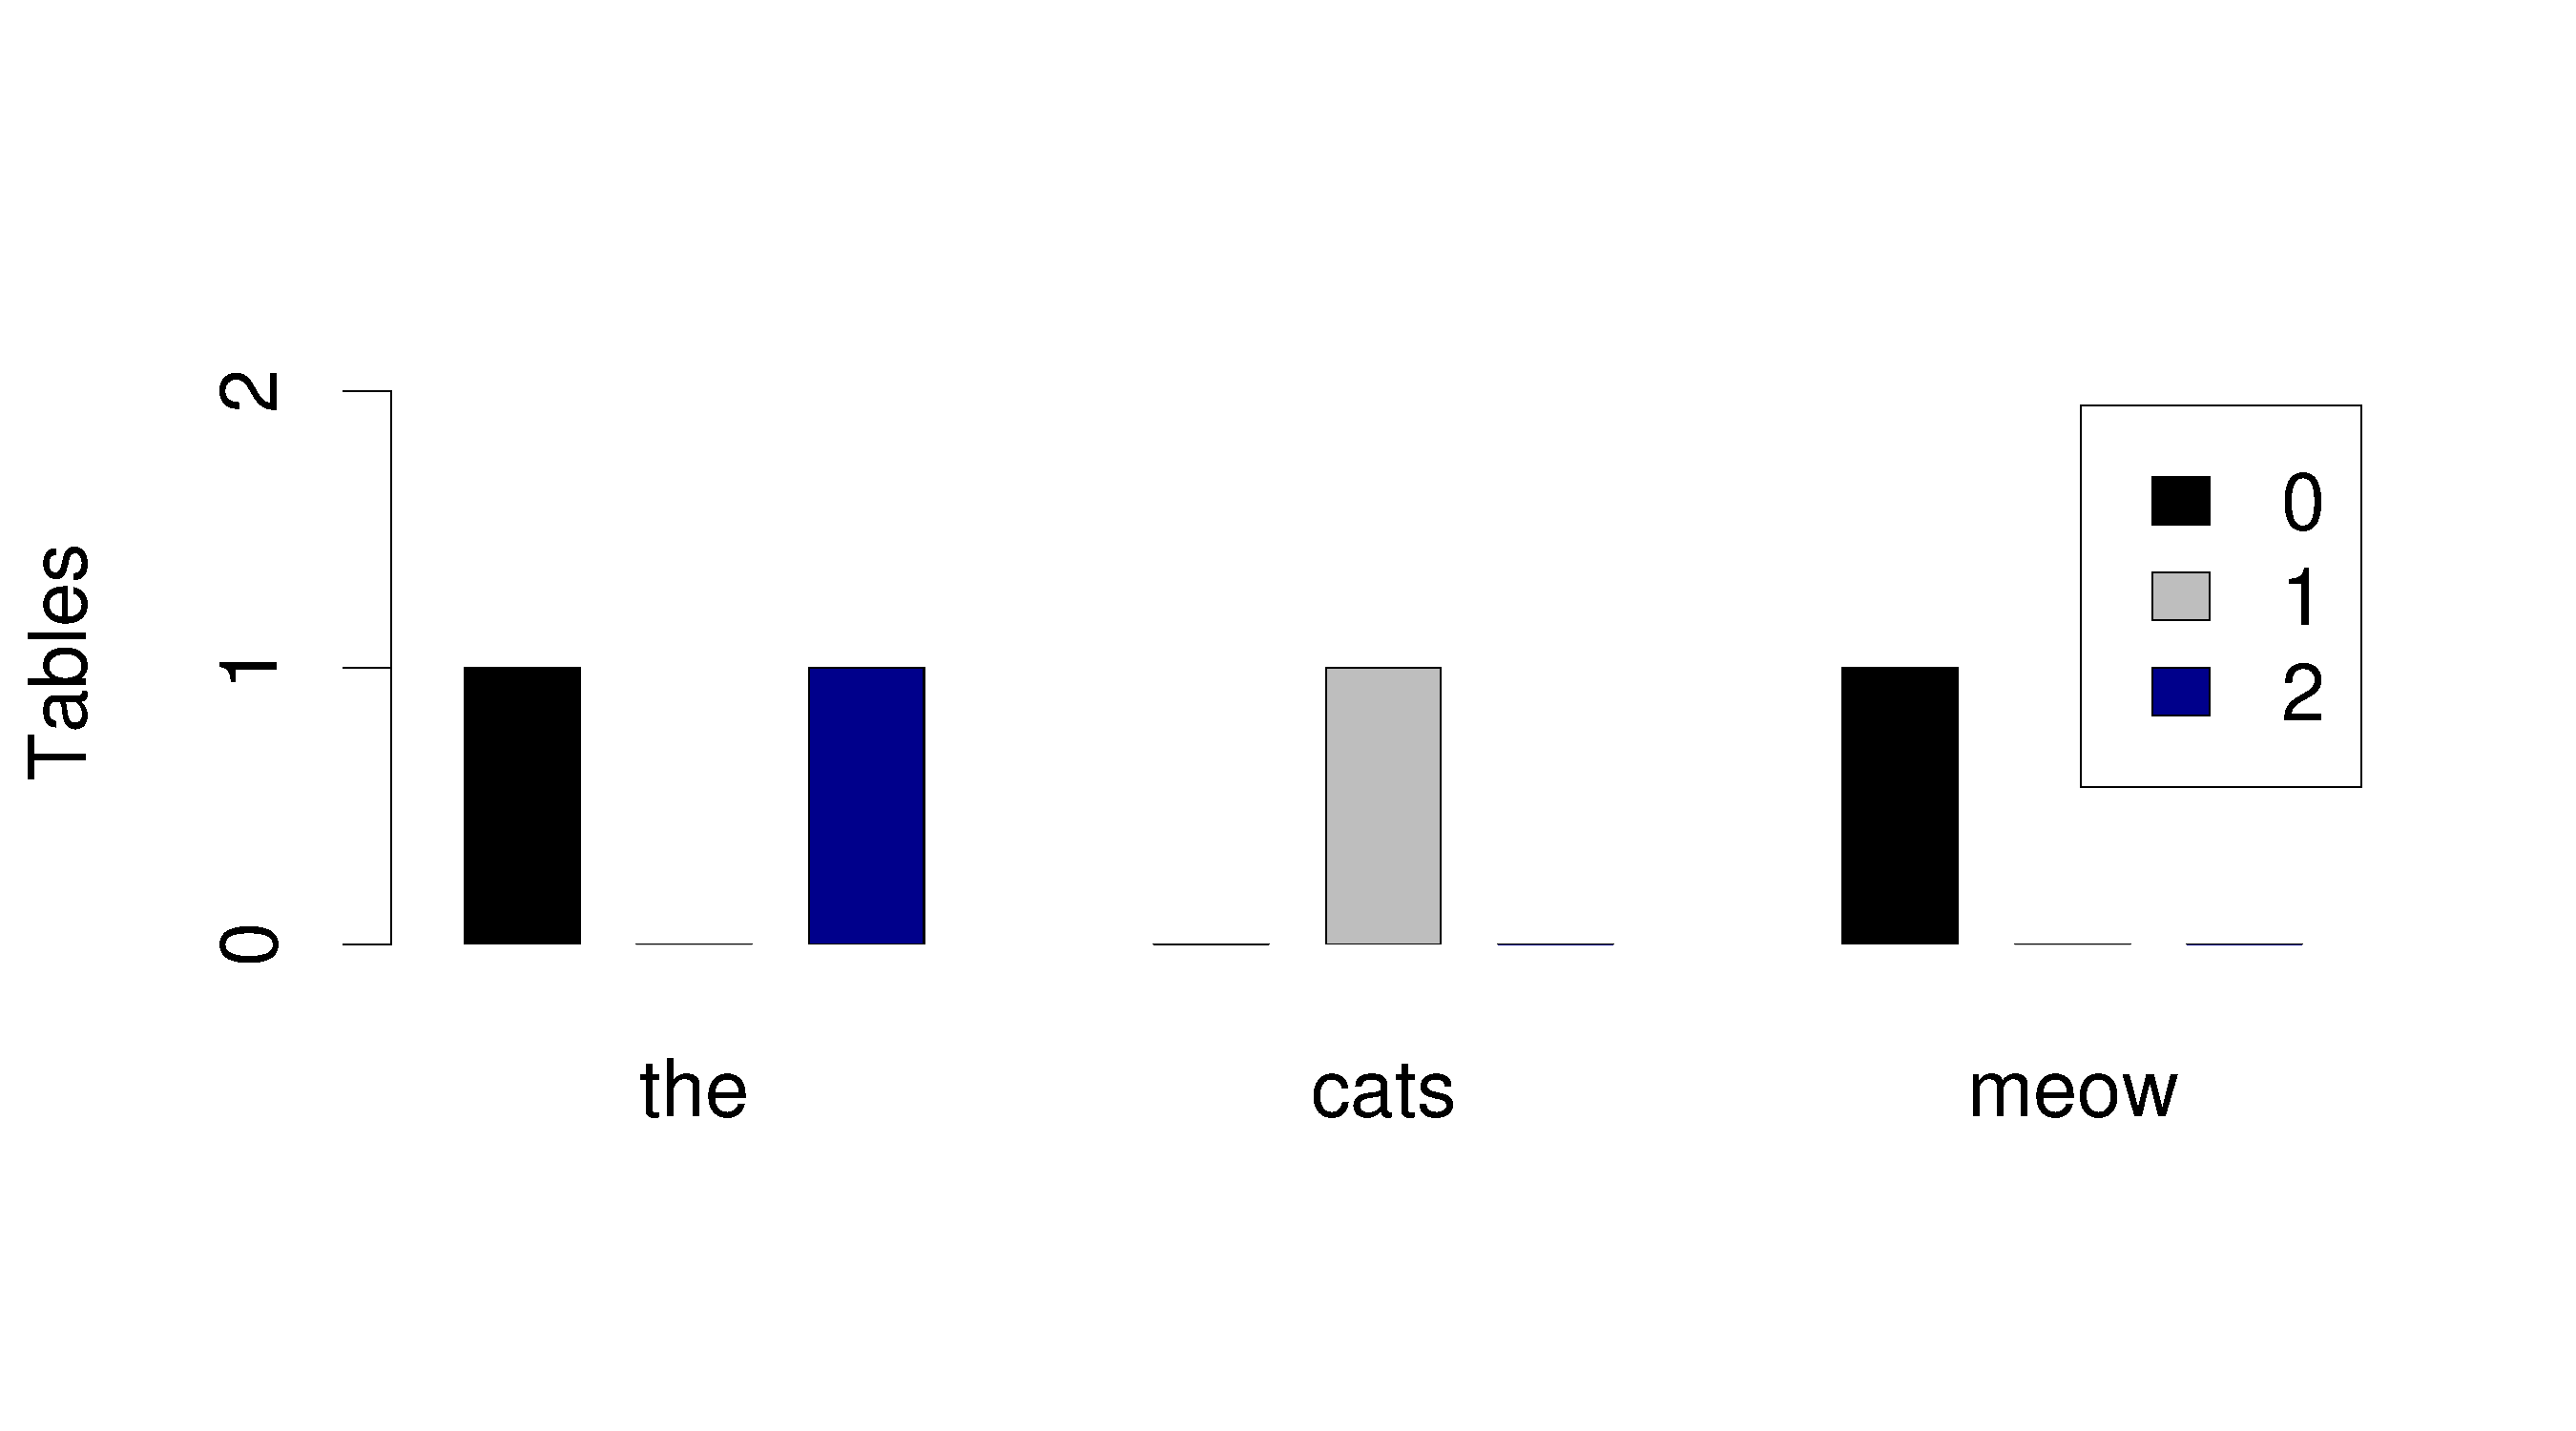
\includegraphics[scale=0.2]{histogram_7.pdf}}
  \only<8>{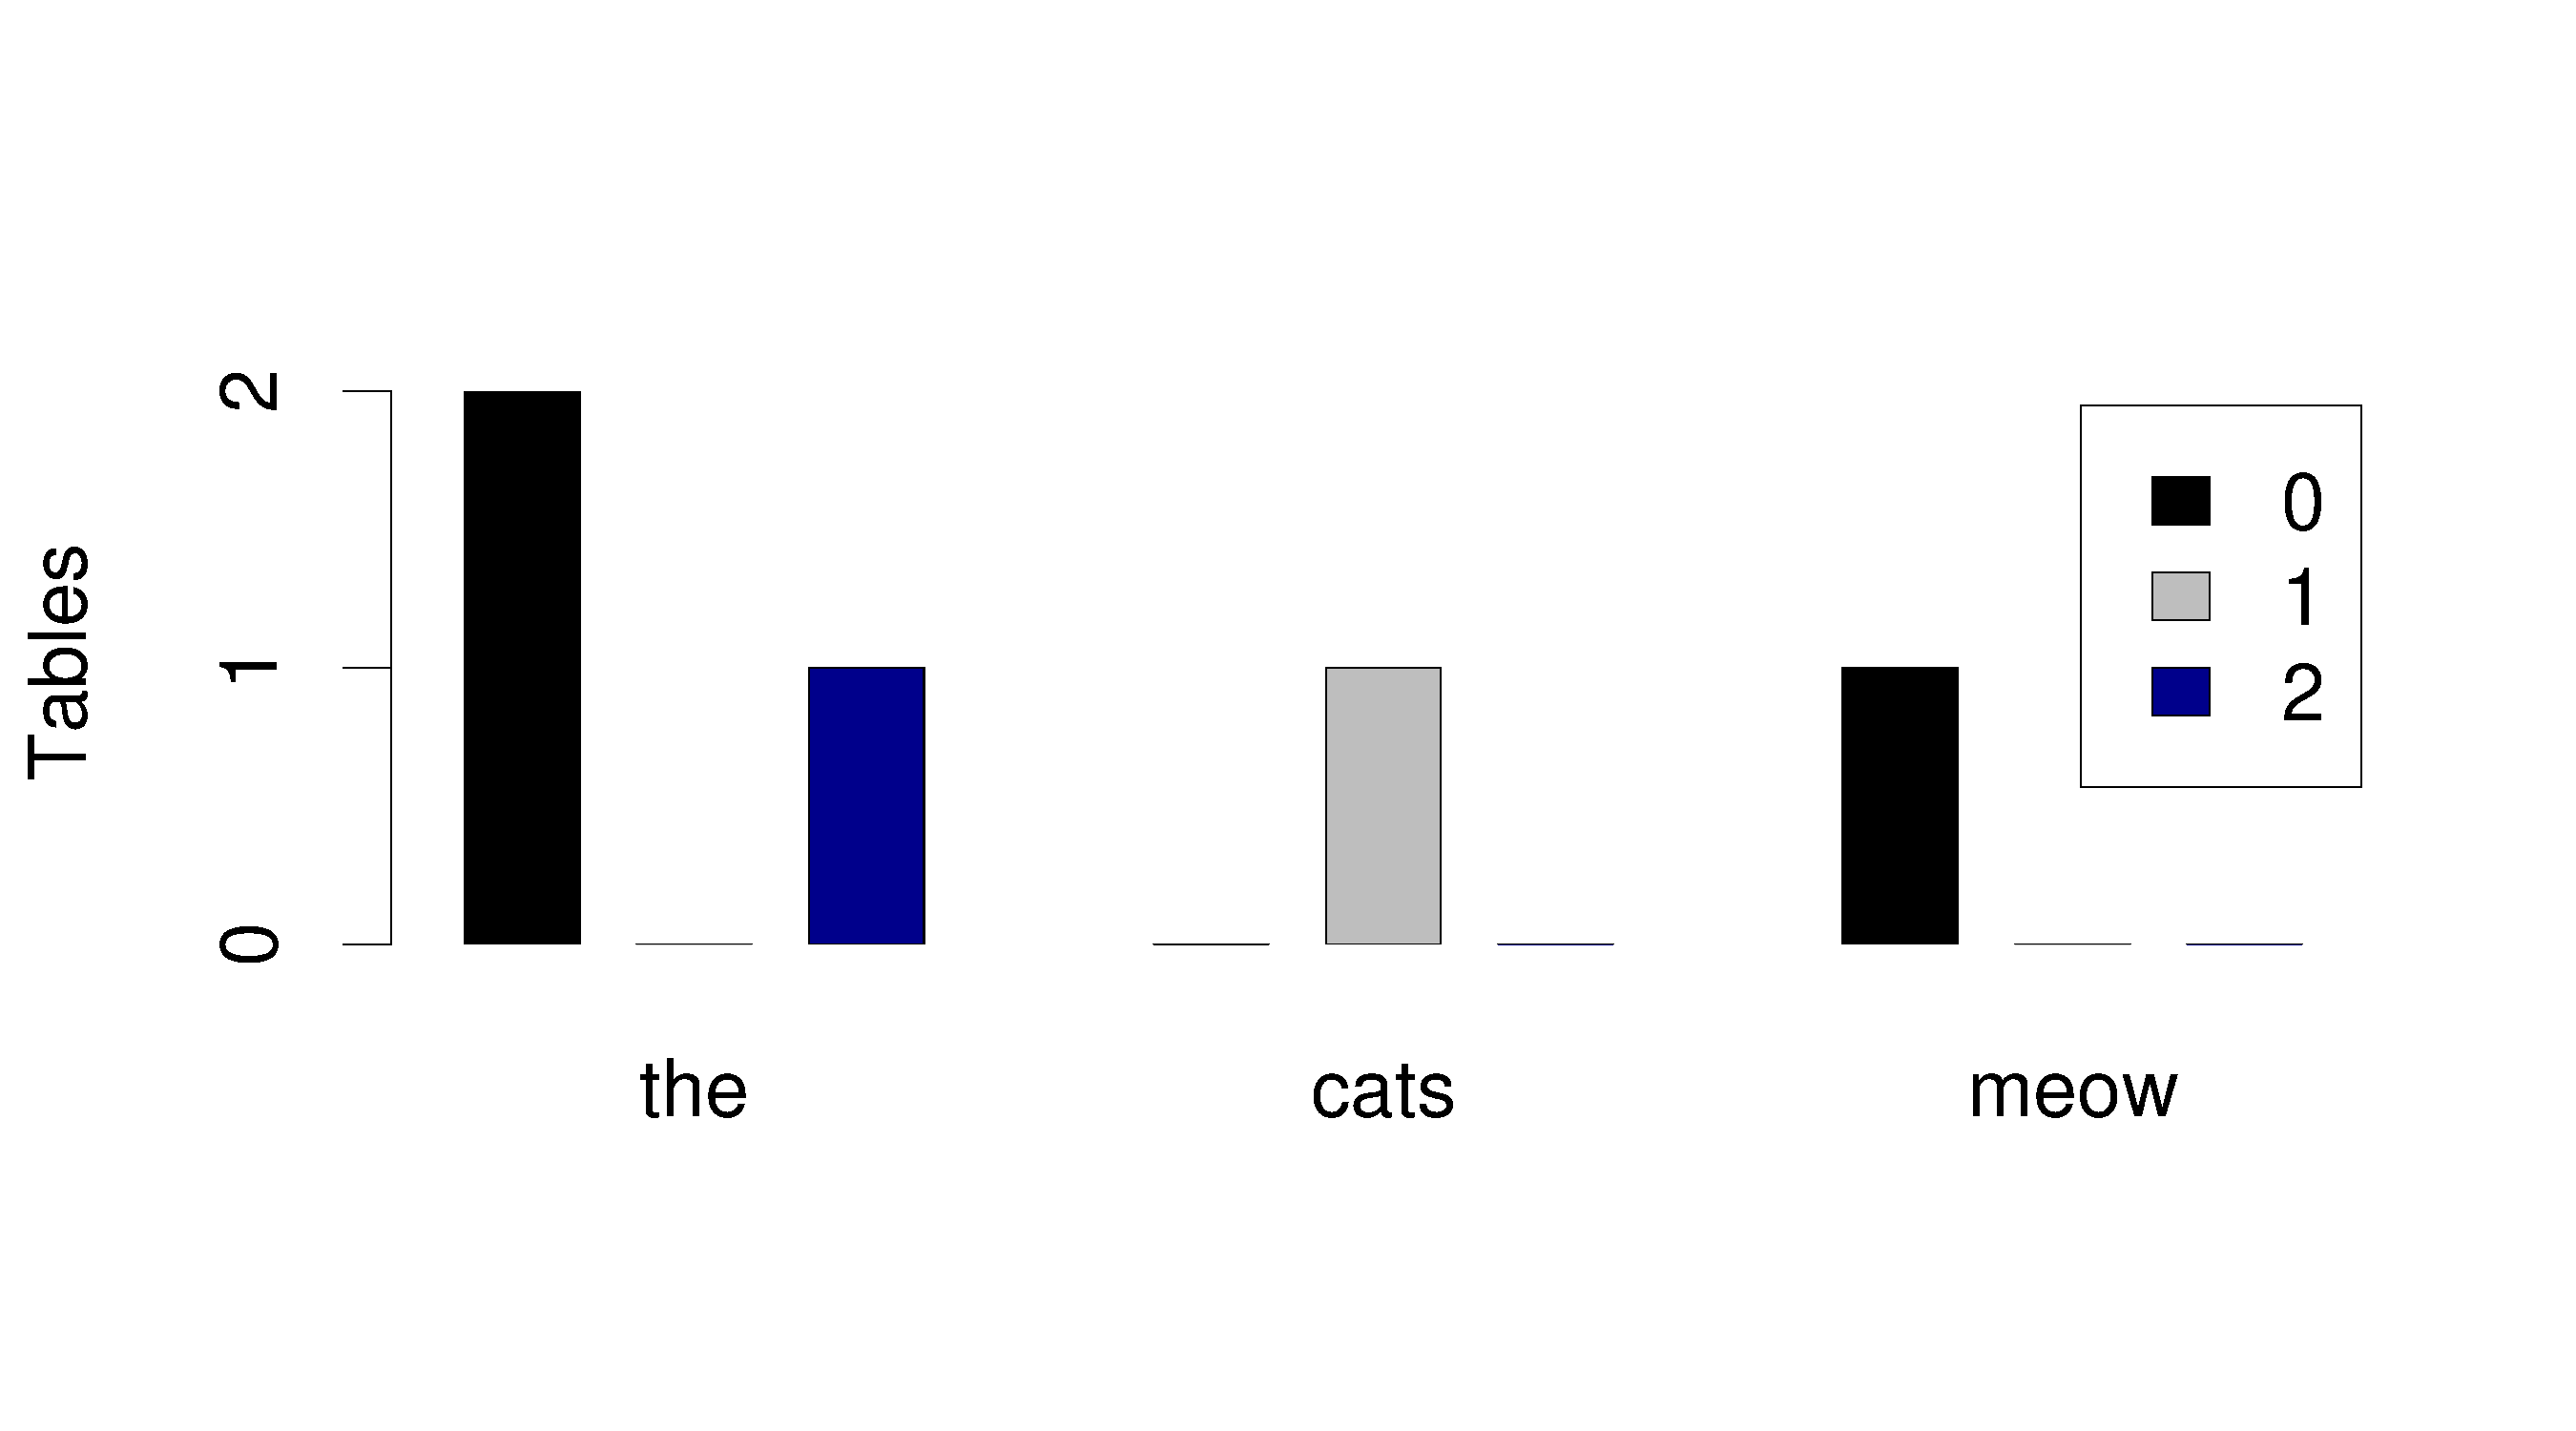
\includegraphics[scale=0.2]{histogram_8.pdf}}
\end{center}
\end{frame}

\begin{frame}
\frametitle{Summary}
\begin{center} 
  \Large \textbf{The table count approximation of Goldwater et al. 2006 
  is broken, \alert{don't use it!}}
\end{center}
\end{frame}

\begin{frame}
%    \frametitle{Summary}
    \begin{center}
        \Large Thank you.
    \end{center}

\begin{block}{References}
    \footnotesize
    \vspace{0.5cm}
    P. Blunsom, T. Cohn, S. Goldwater and M. Johnson. A note on the
    implementation of hierarchical Dirichlet processes,
    {\em In the Proceedings of ACL-IJCNLP 2009}. \\
    \vspace{0.5cm}
    C. E. Antoniak. 1974. Mixtures of dirichlet processes with 
    applications to bayesian nonparametric problems. 
    {\em The Annals of Statistics}, 2(6):1152-1174.  \\
    \vspace{0.5cm}
    S. Goldwater, T. Griffiths, M. Johnson. 
    Contextual dependencies in unsupervised word segmentation. 
    {\em In the Proceedings of (COLING/ACL-2006)}. 
    \vspace{0.5cm}
\end{block}
\end{frame} 

\end{document}
